% Takasuka et al. (2024), A protocol and analysis of year-long simulations of global storm-resolving models and beyond
% Knight et al. (2024), Cloud properties and boundary layer stability above Southern Ocean sea ice and coastal Antarctica
% Zheng et al. (2024), Using Satellite and ARM Observations to Evaluate Cold Air Outbreak Cloud Transitions in E3SM Global Storm-Resolving Simulations
% Schmidt et al. (2024), Effects of vertical grid spacing on the climate simulated in the ICON-Sapphire global storm-resolving model
% Fons et al. (2024), Investigating the sign of stratocumulus adjustments to aerosols in the global storm-resolving model ICON
% Fiddes et al. (2024), A machine learning approach for evaluating Southern Ocean cloud radiative biases in a global atmosphere model
% Mooers et al. (2023), Comparing storm resolving models and climates via unsupervised machine learning
% Zhang et al. (2023), Understanding models' global sea surface temperature bias in mean state: from CMIP5 to CMIP6
% Grundner (2023), Data-Driven Cloud Cover Parameterizations for the ICON Earth System Model Using Deep Learning and Symbolic Regression [thesis]
% Luo et al. (2023), Origins of Southern Ocean warm sea surface temperature bias in CMIP6 models
% Sherriff-Tadano et al. (2023), Southern Ocean Surface Temperatures and Cloud Biases in Climate Models Connected to the Representation of Glacial Deep Ocean Circulation
% Danker et al. (2022), Exploring relations between cloud morphology, cloud phase, and cloud radiative properties in Southern Ocean's stratocumulus clouds
% Possner et al. (2022), Resolution Dependence of Southern Ocean Mixed-Phase Clouds in ICON
% Mauritsen et al. (2022), Early Development and Tuning of a Global Coupled Cloud Resolving Model, and its Fast Response to Increasing CO2
% Wall et al. (2022), Observational Constraints on Southern Ocean Cloud-Phase Feedback
% Grundner et al. (2022), Deep learning based cloud cover parameterization for ICON
% Cesana et al. (2022), Southern Ocean Solar Reflection Biases in CMIP6 Models Linked to Cloud Phase and Vertical Structure Representations
% Fiddes et al. (2022), Southern Ocean cloud and shortwave radiation biases in a nudged climate model simulation: does the model ever get it right?
% Zhao et al. (2022), Compensating Errors in Cloud Radiative and Physical Properties over the Southern Ocean in the CMIP6 Climate Models
% Konsta et al. (2022), Low-Level Marine Tropical Clouds in Six CMIP6 Models Are Too Few, Too Bright but Also Too Compact and Too Homogeneous
% Lin and Yu (2022), The potential impact of model horizontal resolution on the simulation of atmospheric cloud radiative effect in CMIP6 models
% Ramadoss et al. (2021), An evaluation of kilometre scale ICON simulations of mixed-phase stratocumulus over the Southern Ocean durin CAPRICORN [poster]
% Miao et al. (2021), A Regime-based Investigation into the Errors of CMIP6 Simulated Cloud Radiative Effects Using Satellite Observations
% Roh et al. (2021), Intercomparison of cloud properties in DYAMOND simulations over the Atlantic Ocean
% Caldwell et al. (2021), Convection-Permitting Simulations With the E3SM Global Atmosphere Model
% Schuddeboom and McDonald (2021), The Southern Ocean Radiative Bias, Cloud Compensating Errors, and Equilibrium Climate Sensitivity in CMIP6 Models
% Ramadoss et al. (2020), Simulating mixed-phase cloud properties with ICON around the CAPRICORN field campaign at the kilometre scale [poster]
% Heim et al. (2021), Inter-model Variability in Convection-Resolving Simulations of Subtropical Marine Low Clouds
% Seiki and Roh (2020), Improvements in Supercooled Liquid Water Simulations of Low-Level Mixed-Phase Clouds over the Southern Ocean Using a Single-Column Model
% Stevens et al. (2020), The added value of large-eddy and storm-resolving models for simulating clouds and precipitation
% Atlas et al. (2020), How well do large‐eddy simulations and global climate models represent observed boundary layer structures and low clouds over the summertime Southern Ocean?
% Korn et al. (2020), ICON‐O: The Ocean Component of the ICON Earth System Model—Global Simulation Characteristics and Local Telescoping Capability
% Vignesh et al. (2020), Assessment of CMIP6 Cloud Fraction and Comparison with Satellite Observations
% Chen et al. (2022), Evaluation of Simulated Cloud Diurnal Variation in CMIP6 Climate Models
% Jian et al. (2020), Evaluation of the CMIP6 planetary albedo climatology using satellite observations
% Satoh et al. (2019), Global Cloud-Resolving Models
% Hyder et al. (2018), Critical Southern Ocean climate model biases traced to atmospheric model cloud errors

\documentclass[12pt,a4paper]{article}
\usepackage{fontspec}
\usepackage[margin=2cm]{geometry}
\usepackage[citecolor=black]{hyperref}
\usepackage[authoryear,round]{natbib}
\usepackage{doi}
\usepackage{titlesec}
\usepackage{caption}
\DeclareCaptionLabelSeparator{pipe}{ | }
\captionsetup{labelfont={bf,sf},labelsep=pipe}
\usepackage{graphicx}
\setsansfont{Source Sans Pro}
\setmainfont{Source Serif Pro}
\hypersetup{
	colorlinks=true,
	urlcolor=blue,
	pdftitle={Ship and ground-based lidar and radiosonde evaluation of Southern Ocean clouds in the storm-resolving general circulation model ICON and the ERA5 and MERRA-2 reanalyses},
	pdfauthor={Peter Kuma, Frida A.-M. Bender, Adrian J. McDonald and Thorsten Mauritsen}
}
\bibliographystyle{abbrvnat}
\titleformat*{\section}{\large\bfseries\sffamily}
\titleformat*{\subsection}{\normalsize\bfseries\sffamily}
\titlespacing*{\section}{0pt}{12pt}{6pt}
\titlespacing*{\subsection}{0pt}{8pt}{4pt}
%\renewcommand{\bibsection}{\section*{Publications}}
\parskip=6pt
\parindent=0pt

\begin{document}

\begin{center} \Large \sffamily\textbf{Ship and ground-based lidar and radiosonde evaluation of Southern Ocean clouds in the storm-resolving general circulation model ICON and the ERA5 and MERRA-2 reanalyses}\\[0.4cm]
\large Peter Kuma$^\mathsf{1,}$*, Frida A.-M. Bender$^\mathsf{1}$, Adrian J. McDonald$^\mathsf{2}$ and Thorsten Mauritsen$^\mathsf{1}$\\[0.4cm]
\small
$^\mathsf{1}$Department of Meteorology (MISU) and Bolin Centre for Climate Research, Stockholm University, Stockholm SE-106 91, Sweden\\[0.2cm]
$^\mathsf{2}$School of Physical and Chemical Sciences, University of Canterbury, Christchurch, New Zealand\\[0.2cm]
*Corresponding author: Peter Kuma (\href{mailto:peter.kuma@misu.su.se}{peter.kuma@misu.su.se})\\[0.4cm]
\large \today\\[0.4cm]

\end{center}

\section*{Abstract}

Currently, a new generation of km-scale (also called `k-scale') resolution
global climate models is in development as the forthcoming phase of climate
modelling. One such model is a 5-km version of the Icosahedral Nonhydrostatic
Weather and Climate Model (ICON), developed jointly by the Deutscher
Wetterdienst (DWD) and Max-Planck-Institute for Meteorology (MPI-M). Because of
the high resolution, most parametrisations, such as those of convection and
clouds, can be avoided.

Previous studies have identified substantial large-scale biases in model clouds
over the Southern Ocean (SO), affecting sea surface temperature and the Earth's
albedo overall. Our aim is to quantify how well the high-resolution ICON model
is simulating clouds in this region, particularly in light of the fact that
subgrid-scale clouds are not parametrised in this model. This region is mostly
dominated by boundary layer clouds generated by shallow convection, and these
are problematic to observe by spaceborne lidar and radars, which are affected
by attenuation by overlapping and thick clouds and ground clutter,
respectively. Therefore, we choose to use a large set of ship-based
observations conducted with ceilometers and lidars on board of the Research
Vessel (RV) \textit{Polarstern} and other voyages. Altogether, we analyse over
2000 days (about 6 years) of data from 31 voyages and 1 sub-antarctic station
covering diverse longitudes of the SO. To achieve a like-for-like comparison
with the model, we use a ground-based lidar simulator called the Automatic
Lidar and Ceilometer Framework (ALCF). We contrast the results with the ECMWF
Reanalysis 5 (ERA5) and the Modern-Era Retrospective analysis for Research and
Applications, Version 2 (MERRA-2).

We show that the model underestimates the total cloud fraction by about 10\%,
with overestimation of cloud below 2 km and underestimation of cloud above 2
km. The reanalyses also underestimate the total cloud fraction by about 20\%.
ERA5 overestimates cloud below 1 km but underestimates near-surface cloud or
fog. In addition to lidar data, we compare radiosonde profiles acquired on the
RV \textit{Polarstern} voyages with ICON. Notably, the model exhibits smaller
natural variability than observations, and its lifting condensation level tends
to be higher. This might explain why cloud occurrence is peaking higher in the
model (at 500 m) than in observations (at the surface).

The results imply that the SO cloud biases are still a significant issue in a
km-scale resolution model, even though an improvement over the lower-resolution
reanalyses is notable. More effort is needed to improve model cloud simulations
in this fast-changing and understudied region. The advancement from convection
and cloud parametrisation to cloud-resolving models might not solve this bias
without an additional effort.

\section{Introduction}

Increasing climate model resolution is a common way of improving model accuracy
\citep{mauritsen2022}. This is of course limited by the available computational
power and a tradeoff with increasing parametrisation complexity.  Current
computational availability and acceleration from general-purpose computing on
graphics processing units (GPGPUs) is progressing to enable km-scale Earth
system models (ESMs) and coupled atmosphsere--ocean general circulation models
(AOGCMs) in research conditions today and operationally in the forthcoming
years. Therefore, it represents a natural advancement in climate modeling.
Global strom-resolving models (GSRMs) are emerging as a new front in the
development of high-resolution global climate models, with horizontal grid
resolutions of about 2--8 km \citep{satoh2019,stevens2019}. This is enough to
resolve mesoscale convective storms, but smaller-scale convective plumes and
smaller-scale cloud structure remain unresolved. At a 5-km scale,
non-hydrostatic processes also become important, and for this reason such
models are generally non-hydrostatic. The terms global cloud-resolving models
(GCRMs), or global convection-permitting/-resolving models (GCPMs) are also
sometimes used interchangeably with GSRMs but imply that clouds or convection
are resolved explicitly, which is not entirely true for GSRMs, as this would
require an even higher horizontal resolution \citep{satoh2019}.  Representative
of these efforts is the DYnamics of the Atmospheric general circulation Modeled
On Non-hydrostatic Domains (DYAMOND) project \citep{stevens2019,dyamond}, which
is an intercomparison of nine global storm-resolving models (GSRMs) on two
40-day time periods in summer (1 August -- 10 September 2016) and winter (20
January - 1 March 2020). A new one-year GSRM intercomparison is currently
proposed by \cite{takasuka2024}, with the hope of also evaluating the seasonal
cycle and large-scale circulation.  An alternative to using a computantionally
costly GSRM is to train an artificial neural network on GSRM output and use it
for subgrid-scale clouds, as done with the GSRM ICON by \cite{grundner2022};
\cite{grundner2023}.

nextGEMS is an EU-funded project \citep{nextgems} focused on the research and
development of GSRMs at multiple modelling centres and universities in Europe.
The project also develops GSRM versions of the Icosahedral Nonhydrostatic
Weather and Climate Model (ICON), the Integrated Forecasting System (IFS), and
their ocean components at eddy-resolving resolutions: ICON-O coupled with ICON
and Finite-Element/volumE Sea ice-Ocean Model (FESOM) and Nucleus for European
Modelling of the Ocean (NEMO) coupled with IFS.  The project has so far
produced ICON and IFS simulations in three cycles (Cycle 1--3) and pre-final
simulation, with a final production simulation planned by the end of the
project. nextGEMS is not the only project developing GSRMs. Other GSRMs (or
GSRM versions of climate models) currently in development include:
Convection-Permitting Simulations With the E3SM Global Atmosphere Model
[SCREAM; \cite{caldwell2021}], Atmospheric Model [NICAM; \cite{satoh2008}],
Unified Model (UM), eXperimental System for High-resolution modeling for
Earth-to-Local Domain [X-SHiELD; \cite{shield}], Action de Recherche Petite
Echelle Grande Echelle-NonHydrostatic version [ARPEGE-NH;
\cite{bubnova1995,voldoire2017}], Finite-Volume Dynamical Core on the Cubed
Sphere [FV3, \cite{lin2004}], NASA Goddard Earth Observing System global
atmospheric model version 5 [GEOS5; \cite{putman2011}], Model for Prediction
Across Scales [MPAS; \cite{skamarock2012}], and System for Atmospheric Modeling
[SAM; \cite{khairoutdinov2003}].

Multiple cloud properties have an effect on the shortwave (SW) and longwave
(LW) radiation. On the first order, it is the total cloud fraction, cloud
phase, and the liquid and ice water path. These are influenced by the
atmopheric thermodynamics, convection and circulation, and indirect and direct
effects of aerosols. On smaller orders, it is the cloud droplet size
distribution, ice crystal habit, cloud lifetime, and direct radiative
interaction with aerosols.  In the 6th phase of the Coupled Model
Intercomparison Project [CMIP6; \citep{eyring2016}], the cloud feedback has
increased relative to CMIP5 \citep{zelinka2020}, also being one of the main
reasons for the higher climate sensitivity of CMIP6 models.

The Southern Ocean (SO) is known to be a problematic region for climate model
biases due to reasons such as a lack of surface and in situ observations and
being a lower priority region for numerical weather prediction (NWP) and
climate model development because it is far away from populated areas of
interest.  Nevertheless, radiation biases and changes over an area of its size
have a very significant influence on the global climate, and the SO is an
important part of the global ocean conveyor belt.  Marine clouds have
disproportionate effect on top of atmosphere (TOA) SW radiation due to the
relatively low albedo of the sea surface.  The longitudinal symmetry of the SO
means that model cloud biases tend to be similar across longitudes.  Here, we
will conventionally refer to the SO as ocean regions south of 40°S,
low-latitude SO as 40--55°S and high-latitude SO as south of 55°S.

SO radiation biases have been relatively large and systematic compared to the
rest of the globe since at least CMIP3 \citep{trenberth2010}, and the SO SW CRE
bias is still positive in eight analysed CMIP6 models analysed by
\cite{schuddeboom2021} over high-latitude SO, whereas over low-latitude SO it
tends to be more neutral or negative in some models. Too much absorbed SW
radiation over the SO was also identified in the GSRM SCREAM
\cite{caldwell2021}. Compensating biases are possible, such as the `too few too
bright' cloud bias, characterised by too small cloud fraction and too large
cloud albedo \citep{wall2017,kuma2020}, previously described by
\cite{webb2001}, \cite{weare2004}, \cite{zhang2005}, \cite{karlsson2008},
\cite{nam2012}, \cite{klein2013}, and \cite{bender2017} in other regions and
models. That is, a model maintains a resonable SW radiation balance by
reflecting too much SW radiation by cloudy sky but has too little cloudy sky
area overall. A study by \cite{konsta2022} showed that this type bias is still
present in six analysed CMIP6 models in tropical marine clouds, using the
GCM-Oriented Cloud-Aerosol Lidar and Infrared Pathfinder Satellite Observation
(CALIPSO) Cloud Product [CALIPSO--GOCCP; \cite{chepfer2010}] and Polarization
\& Anisotropy of Reflectances for Atmospheric Sciences coupled with
Observations from a Lidar [PARASOL; \citep{lier2008}] as a reference. They
suggest improper simulation of subgrid-scale cloud heterogeneity as a cause.
Compensating cloud biases in the Australian Community Climate and Earth System
Simulator (ACCESS) – Atmosphere-only model version 2 (AM2) over the SO were
analysed by \cite{fiddes2022} and \cite{fiddes2024}.  \cite{possner2022} showed
that over the SO, the DYAMOND GSRM ICON underestimates low-level cloud fraction
on the order of 30\% [relative to the Moderate Resolution Imaging
Spectroradiometer (MODIS)] and overestimates downwelling TOA SW radiation on
the order of 10 Wm$^\mathrm{-2}$ in  [relative to the Clouds and the Earth’s
Radiant Energy System (CERES)] in the highest model resolution run (2.5 km).
\cite{zhao2022} reported a similar SW radiation bias in five analysed CMIP6
models over high-latitude SO and total CF underestimation on the order of 10\%
over the entire 40--60°S SO.

In general, SST biases in the SO can originate either in the atmosphere, caused
by too much shortwave heating of the surface, too little longwave cooling of
the surface, or in the ocean circulation.  Interactions of both are also
possible, due to, for example SST affecting clouds and clouds affecting the
surface radiation.  \cite{zhang2023} have shown that SST biases have improved
in CMIP6 compared to CMIP5 (relative to ERA5), with SST overall increasing in
the later CMIP phase. However, over the SO this resulted in an even higher
positive bias, especially in the Atlantic Ocean (AO) sector of the SO,
increasing by up to 1°C.  \cite{luo2023} identified that the SO SST bias in an
ensemble of 18 CMIP6 models originates not from the surface heat and radiation
fluxes (using reanalyses as a reference), but from a warm bias in the Northern
Atlantic Deep Water.

The main aim of our research is to evaluate the GSRM version of ICON, developed
jointly by nextGEMS, Deutscher Wetterdienst (DWD) and the Max-Planck-Institute
for Meteorology (MPI-M). Previous studies have identified substantial
large-scale biases in climate model clouds over the Southern Ocean (SO),
affecting sea surface temperature and the Earth’s albedo overall. Our aim is to
quantify how well the high-resolution ICON model is simulating clouds in this
region, particularly in light of the fact that subgrid-scale clouds are not
parameterised in this model. This region is mostly dominated by boundary layer
clouds generated by shallow convection, and these are problematic to observe by
spaceborne lidar and radars, which are affected by attenuation by overlapping
and thick clouds and ground clutter, respectively.  Specifically, the radar on
CloudSat and lidar on CALIPSO are affected by the abovementioned issues,
resulting in a strong underestimation of cloud occurrence below 2 km relative
to ground-based lidar observations \citep{mcerlich2021}.  This, in turn, can
lead to systematic biases in low clouds in climate models, which are frequently
evaluated against CloudSat--CALIPSO products. Reanalyses can also suffer from
cloud biases, as these are usually parametrised in their atmospheric component,
and also in regions where input observations are sparse.  This makes them a
problematic reference for clouds over the SO, and any biases relative to a
reanalysis should be interpreted with caution. Instead, we chose to use a large
set of ship-based observations conducted with ceilometers and lidars on board
of the RV \emph{Polarstern} and other voyages and stations as a reference for
the model evaluation.

Altogether, we analysed over 1500 days of data from 31 voyages and one
sub-Antarctic station covering diverse longitudes of the SO. To achieve a
like-for-like comparison with the model, we used a ground-based lidar simulator
called the Automatic Lidar and Ceilometer Framework (ALCF) \citep{kuma2021}. We
contrasted the results with the European Centre for Medium-Range Weather
Forecasts (ECMWF) Reanalysis 5 (ERA5) \citep{era5} and the Modern-Era
Retrospective analysis for Research and Applications, Version 2 (MERRA-2)
\citep{gelaro2017}.

\begin{figure}
\centering
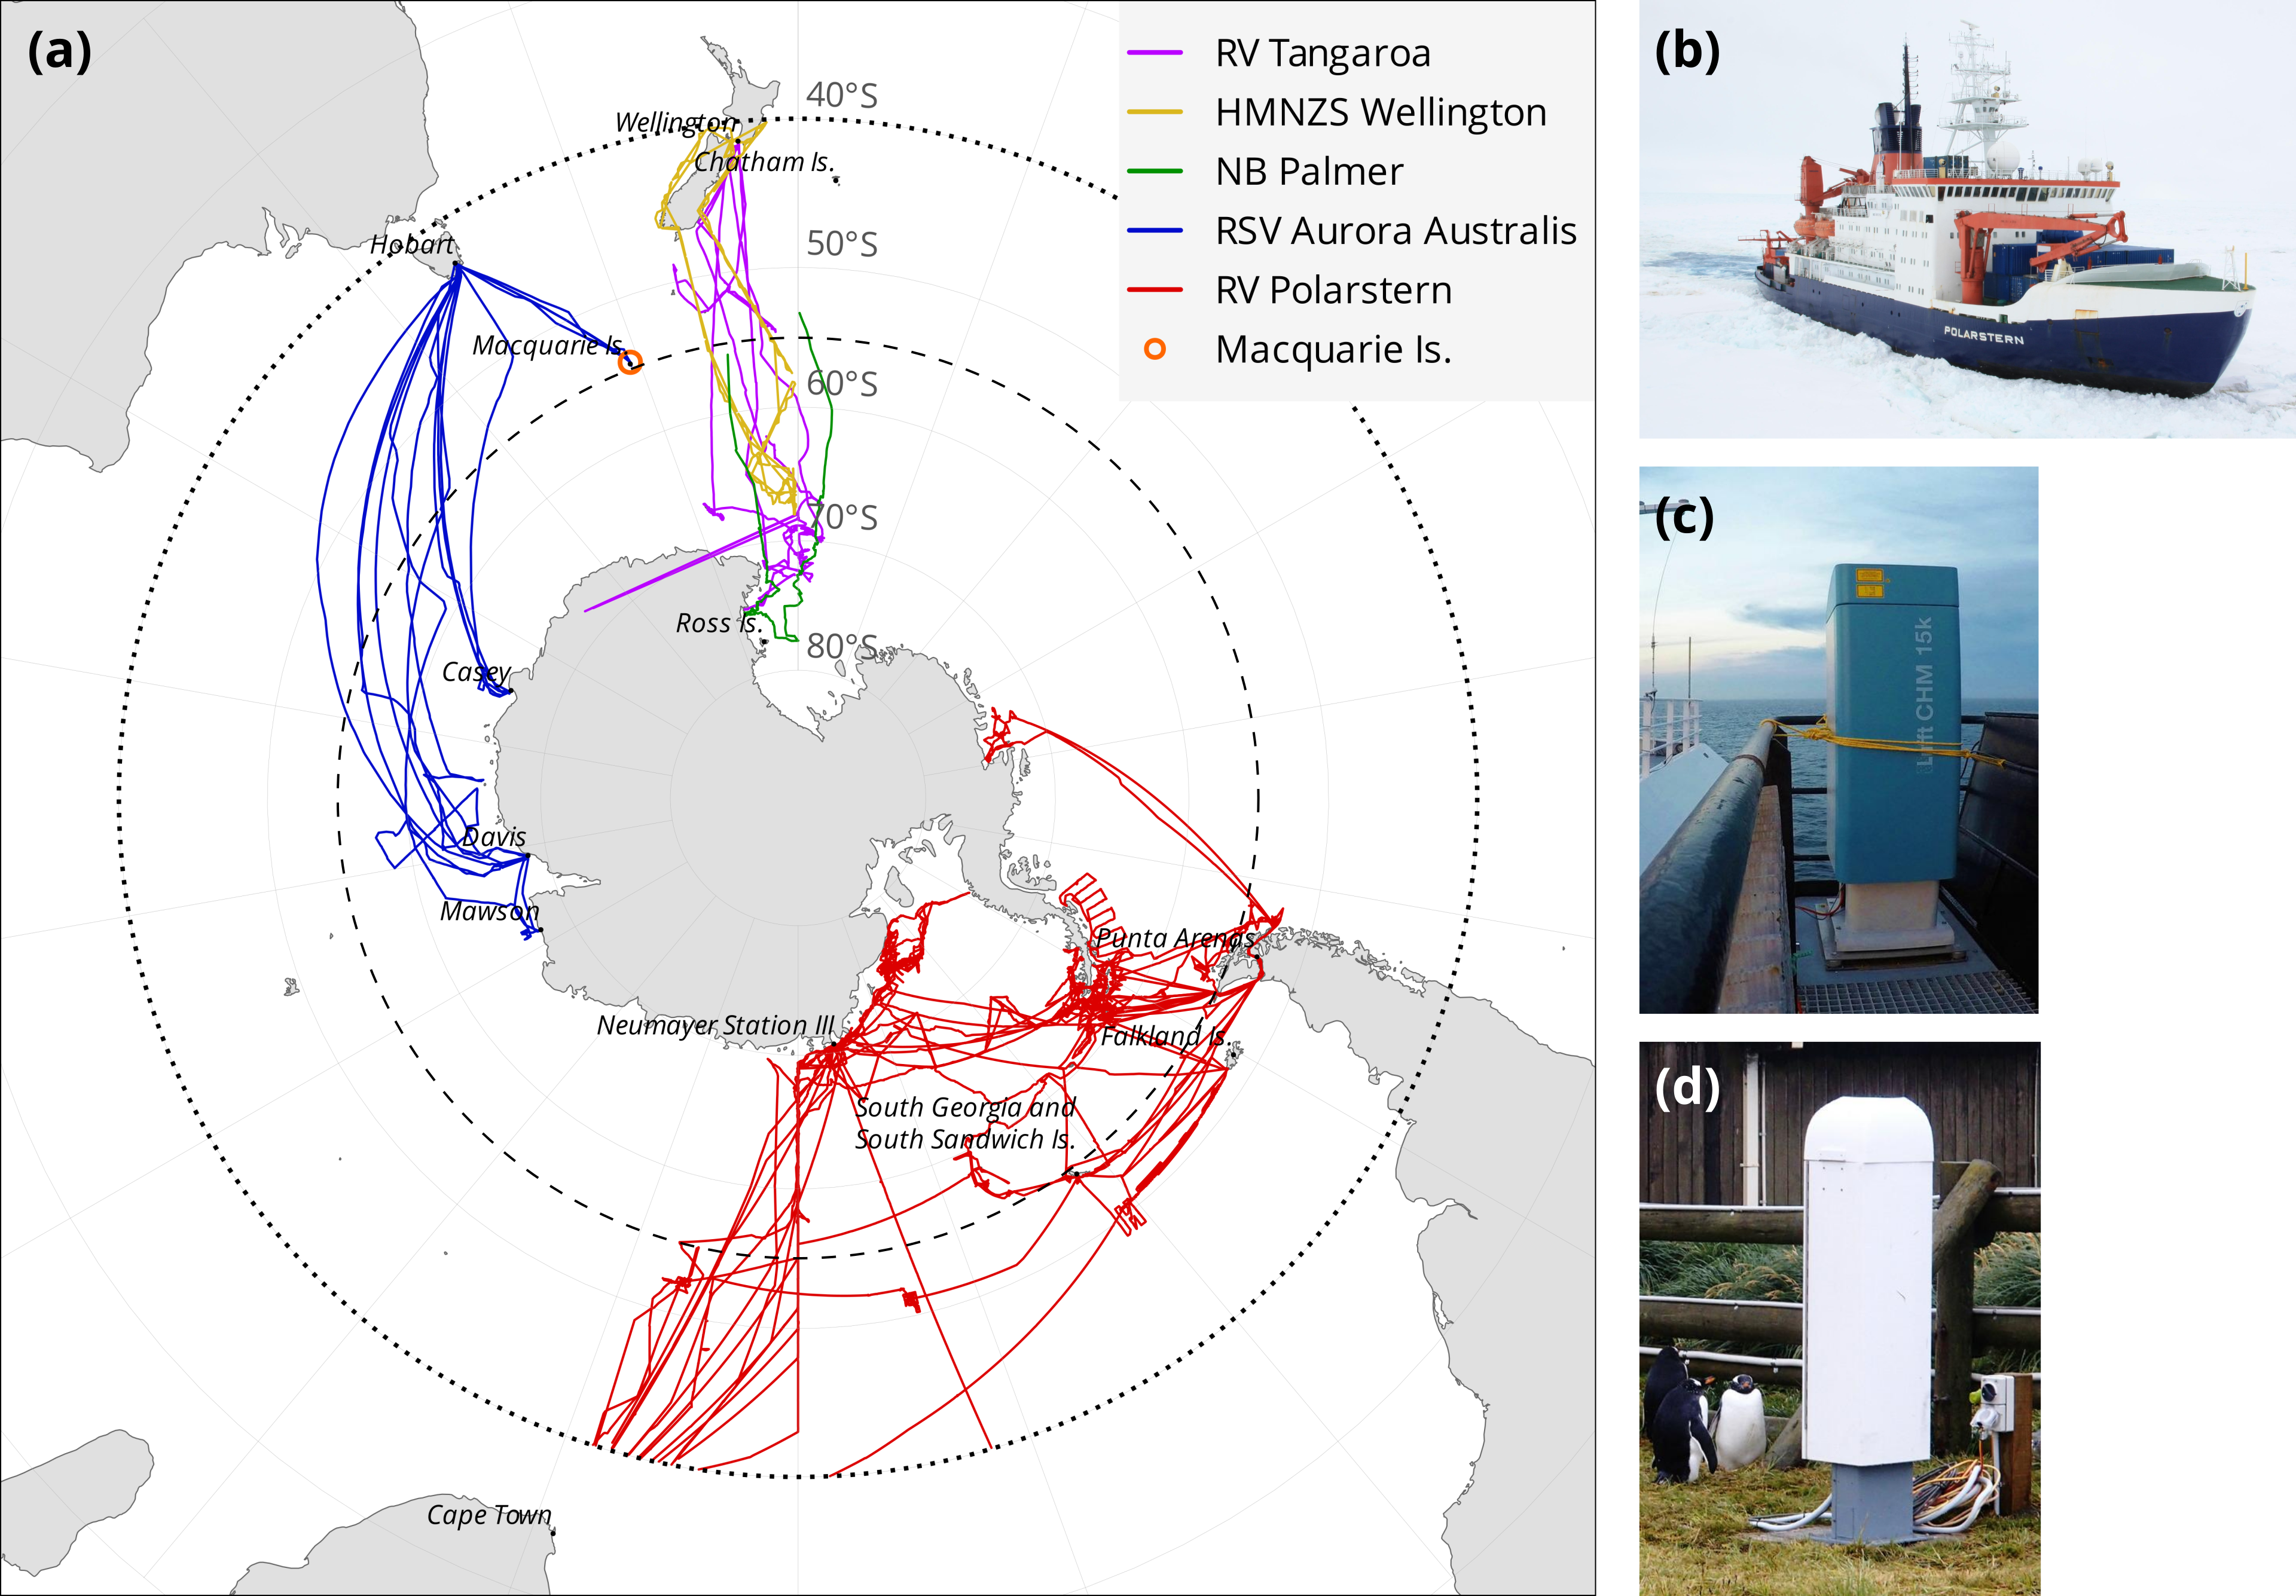
\includegraphics[width=\textwidth]{img/map_fig.pdf}
\caption{
\textbf{(a)} A map showing the tracks of 31 voyages of RV \emph{Polarstern},
RSV \emph{Aurora Australis}, RV \emph{Tangaroa}, RV \emph{Nathaniel B. Palmer},
and HMNZS \emph{Wellington} and one sub-Antarctic station (Macquarie Island)
analysed here. The tracks cover Antarctic sectors south of South America, the
Atlantic Ocean, Africa, Australia, and New Zealand in the years 2010--2021
(inclusive).  The dotted and dashed lines at 40°S and 55°S delineate the
Southern Ocean area of our analysis and its partitioning into two subsets,
respectively.  A photo of \textbf{(b)} RV \emph{Polarstern} (© Folke Mehrtens,
Alfred-Wegener-Institut), \textbf{(c)} Lufft CHM 15k installed on RV
\emph{Tangaroa} (© Peter Kuma, University of Canterbury), \textbf{(d)} Vaisala
CL51 installation at the Macquarie Island station (© Jeff Aquilina, Bureau of
Meteorology).
% TODO: Ask for photo permission and info about license.
}
\label{fig:map}
\end{figure}

\begin{figure}
\centering
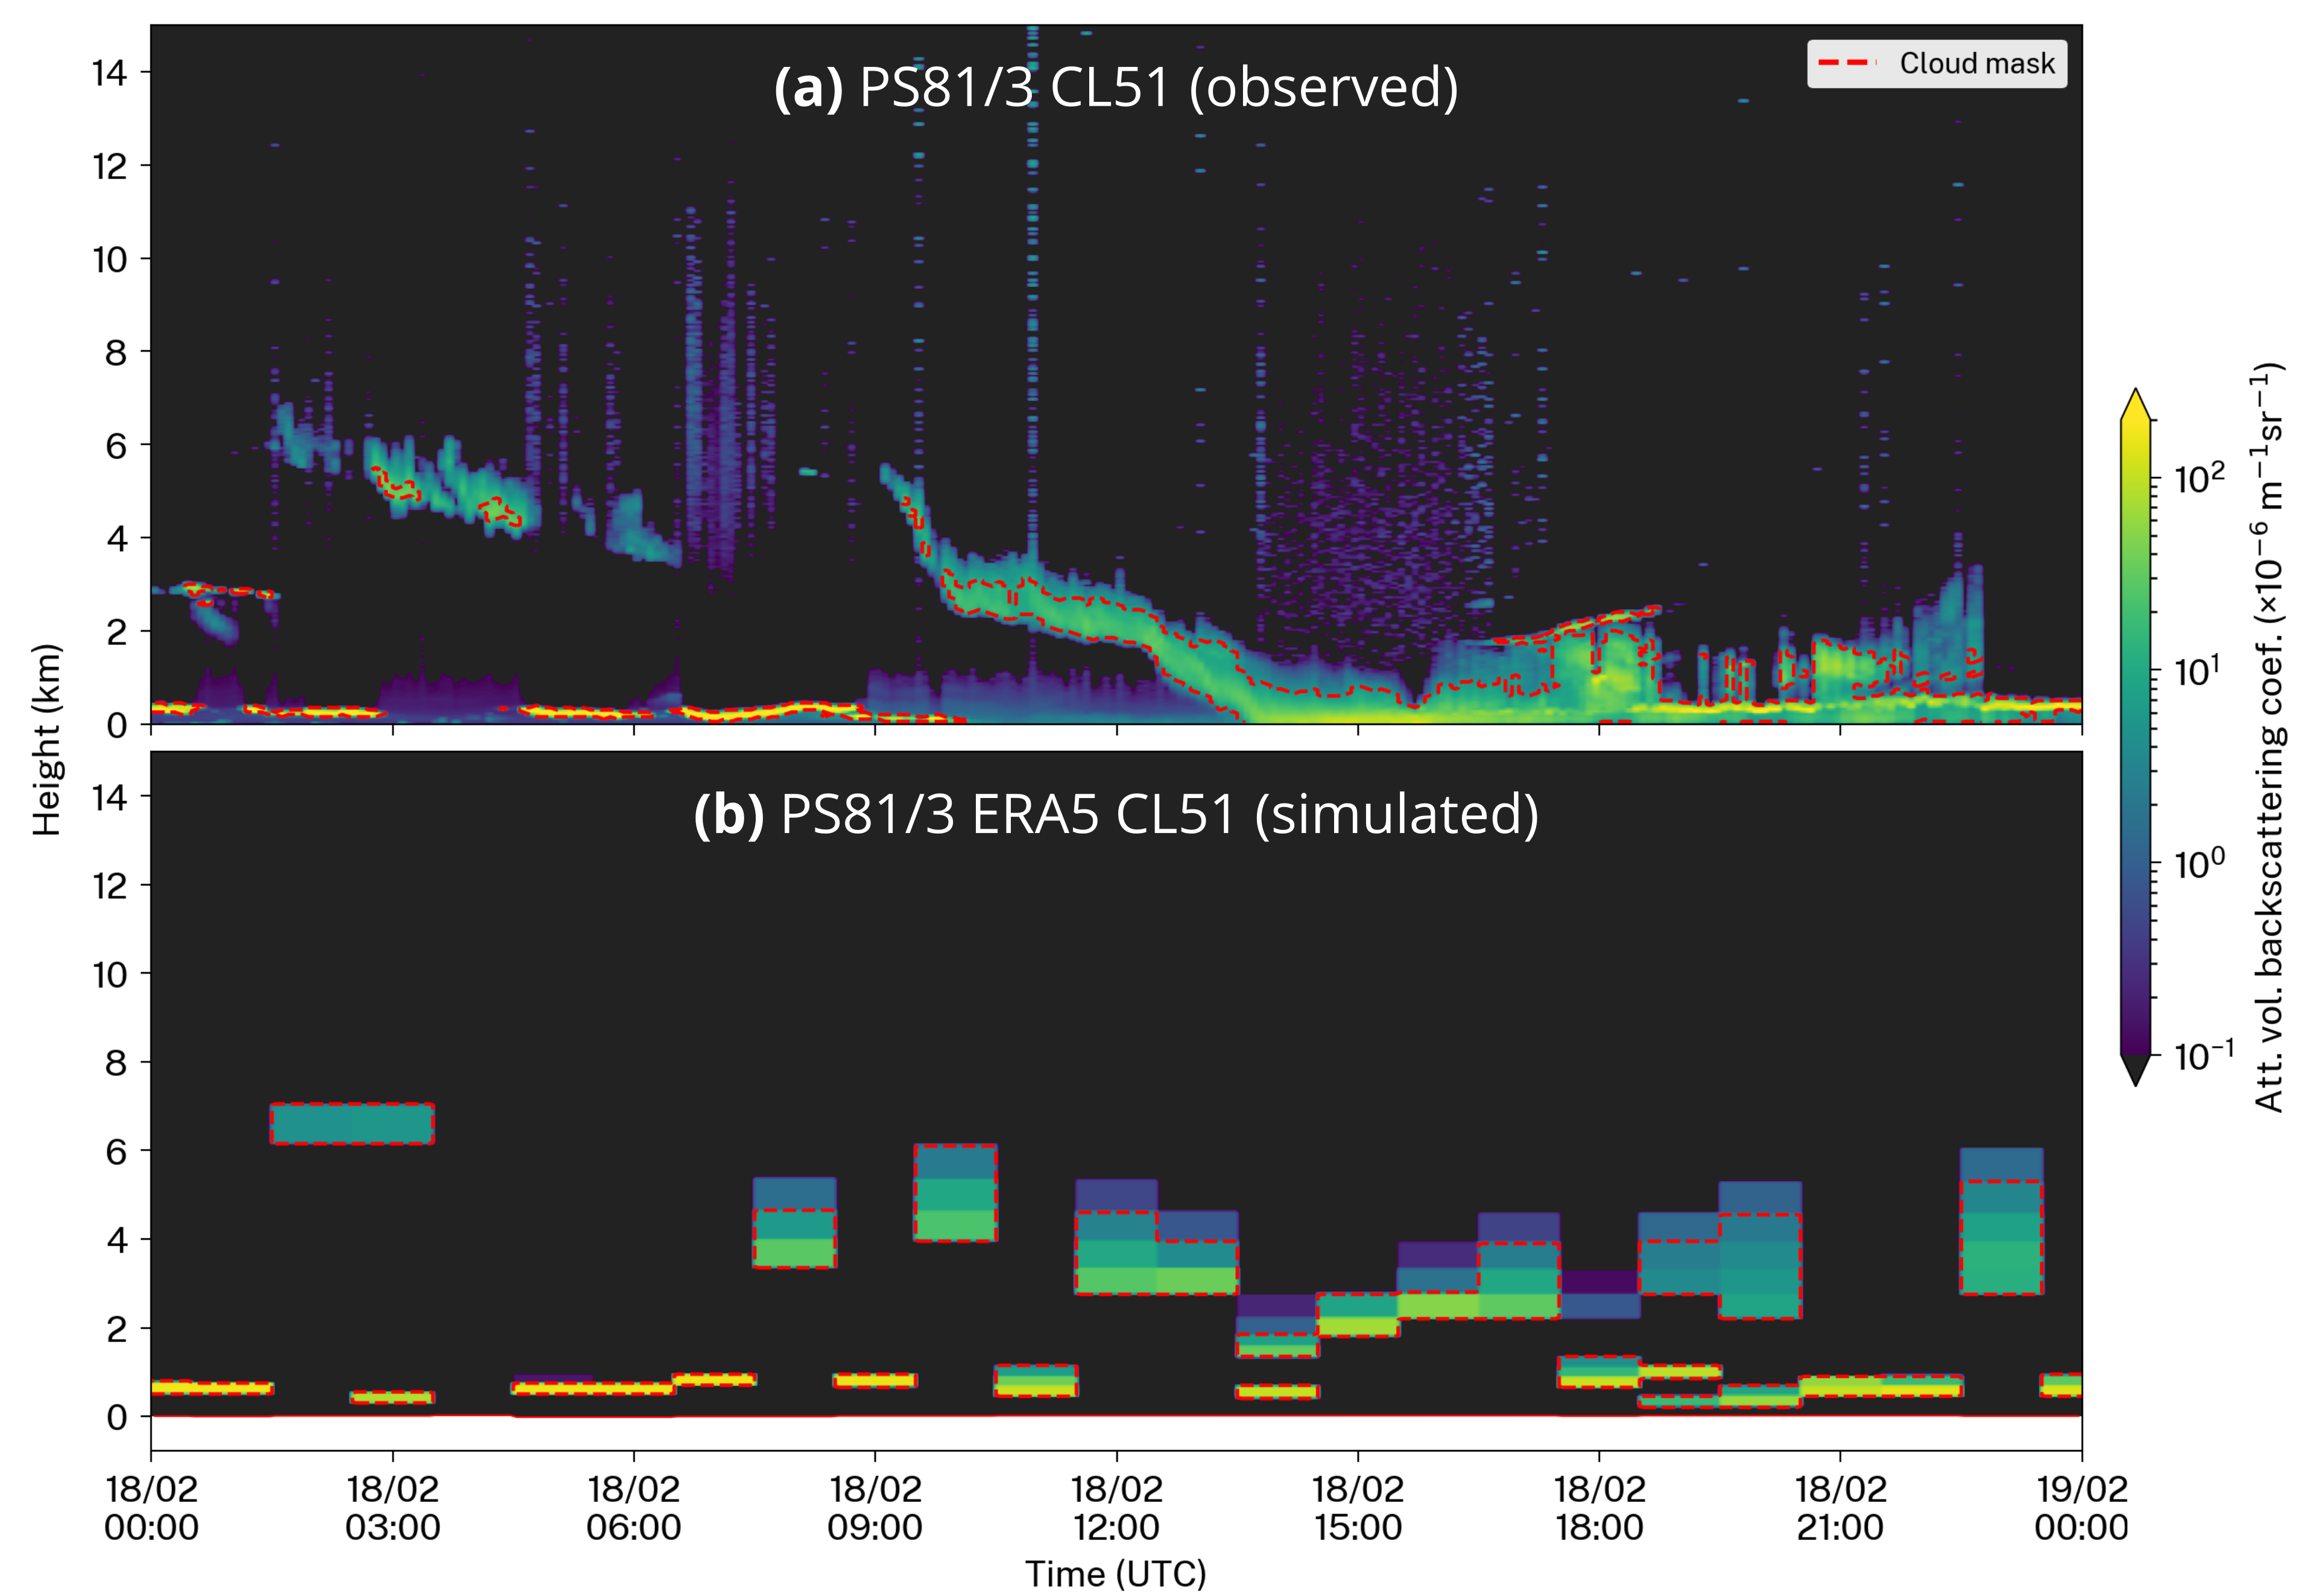
\includegraphics[width=\textwidth]{img/example.png}
\caption{
An example of attenuated volume backscattering coefficient (AVBC) \textbf{(a)}
measured by CL51 during 24 hours on the PS81/3 voyage and \textbf{(b)} an
equivalent AVBC simulated with the ALCF from ERA5 data during the same time
period. Shown is also the cloud mask determined by the ALCF.
}
\label{fig:example}
\end{figure}

\begin{figure}
\centering
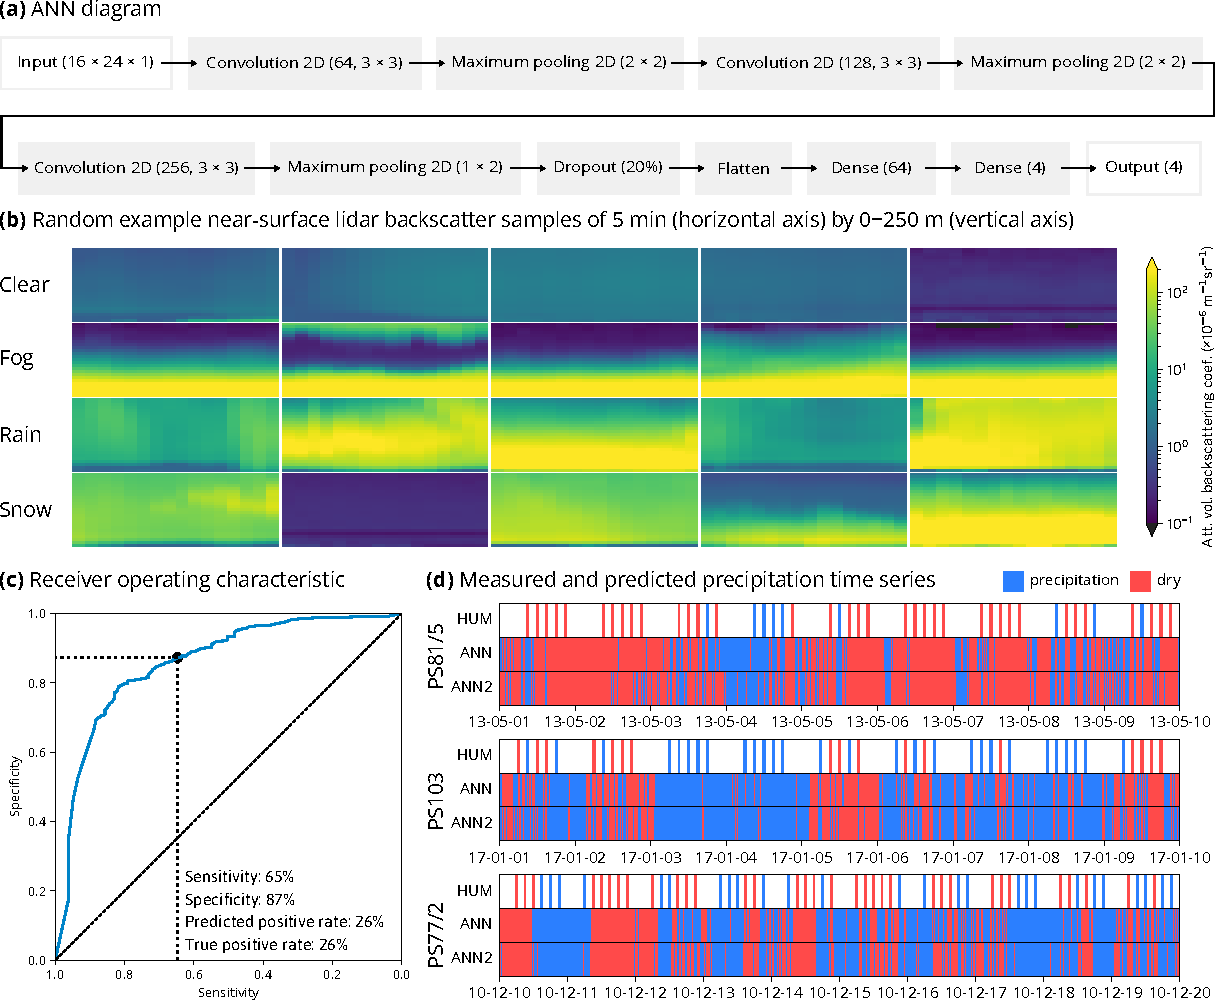
\includegraphics[width=\textwidth]{img/ann.pdf}
\caption{
Artificial neural network (ANN) for prediction of precipitation in lidar
backscatter. \textbf{(a)} Diagram showing the TensorFlow structure of the ANN,
\textbf{(b)} randomly selected example samples of near-surface backscatter in
four categories (clear, fog, rain and snow), as determined by coincident
human-performed weather observations, \textbf{(c)} receiver operating
characteristic diagram of the ANN, \textbf{(d)} examples of 10-day time series
of human-observed (`HUM') and predicted precipitation based on an ANN trained
on all voyages (`ANN') and all voyages except for the shown voyage (`ANN2')
during three randomly selected voyages with the available data. Here, by
`randomly selected' we mean selected from the top of a permutation generated by
a pseudo-random number generator to prevent authors' bias in the selection.
}
\label{fig:ann}
\end{figure}

\begin{figure}
\centering
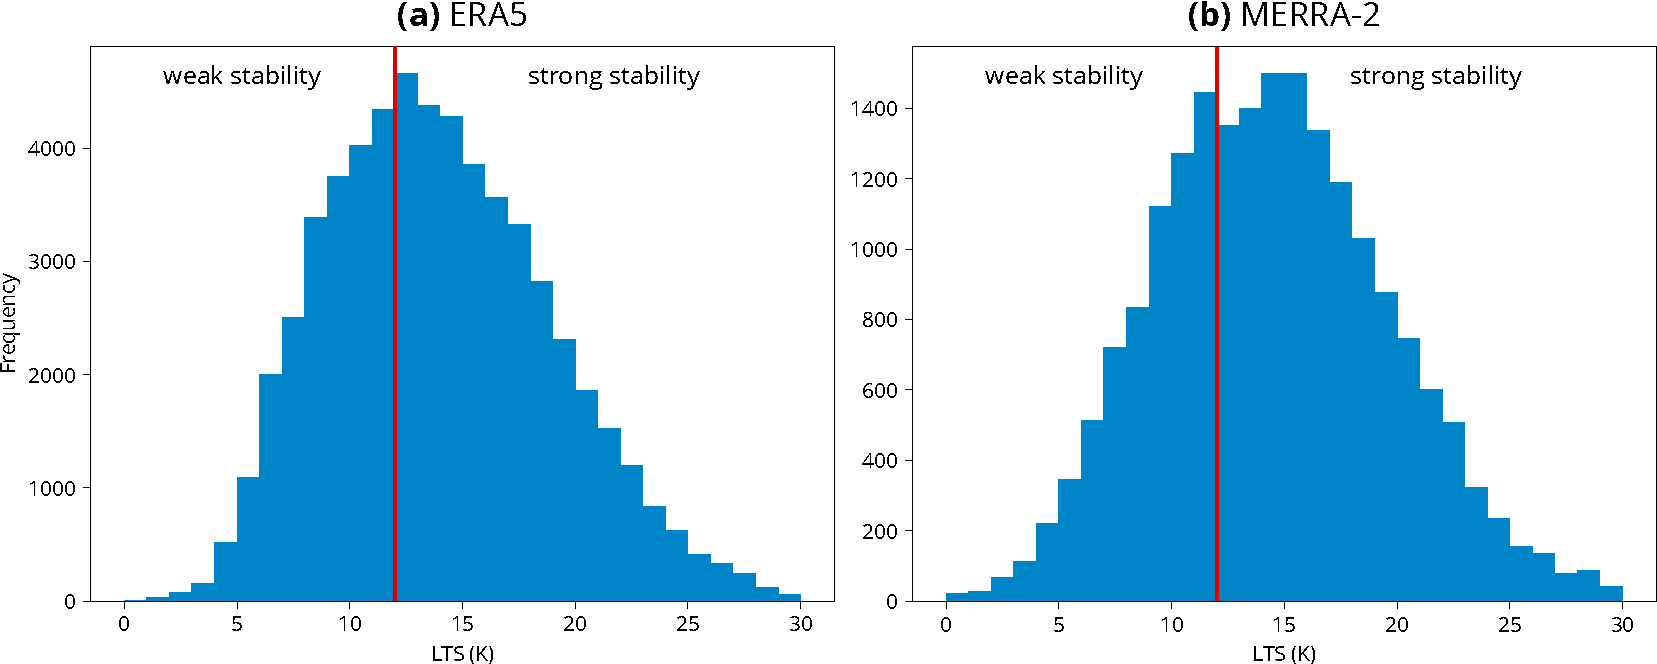
\includegraphics[width=\textwidth]{img/lts_dist.pdf}
\caption{
Lower tropospheric stability (LTS) distribution in \textbf{(a)} ERA5 and
\textbf{(b)} MERRA-2 calculated for the 31 voyage tracks and one station from
the highest instantaneous temporal resolution data available. Shown is also the
chosen dividing threshold of 12 K for `stable' and `unstable' conditions.
}
\label{fig:lts}
\end{figure}

\begin{figure}
\centering
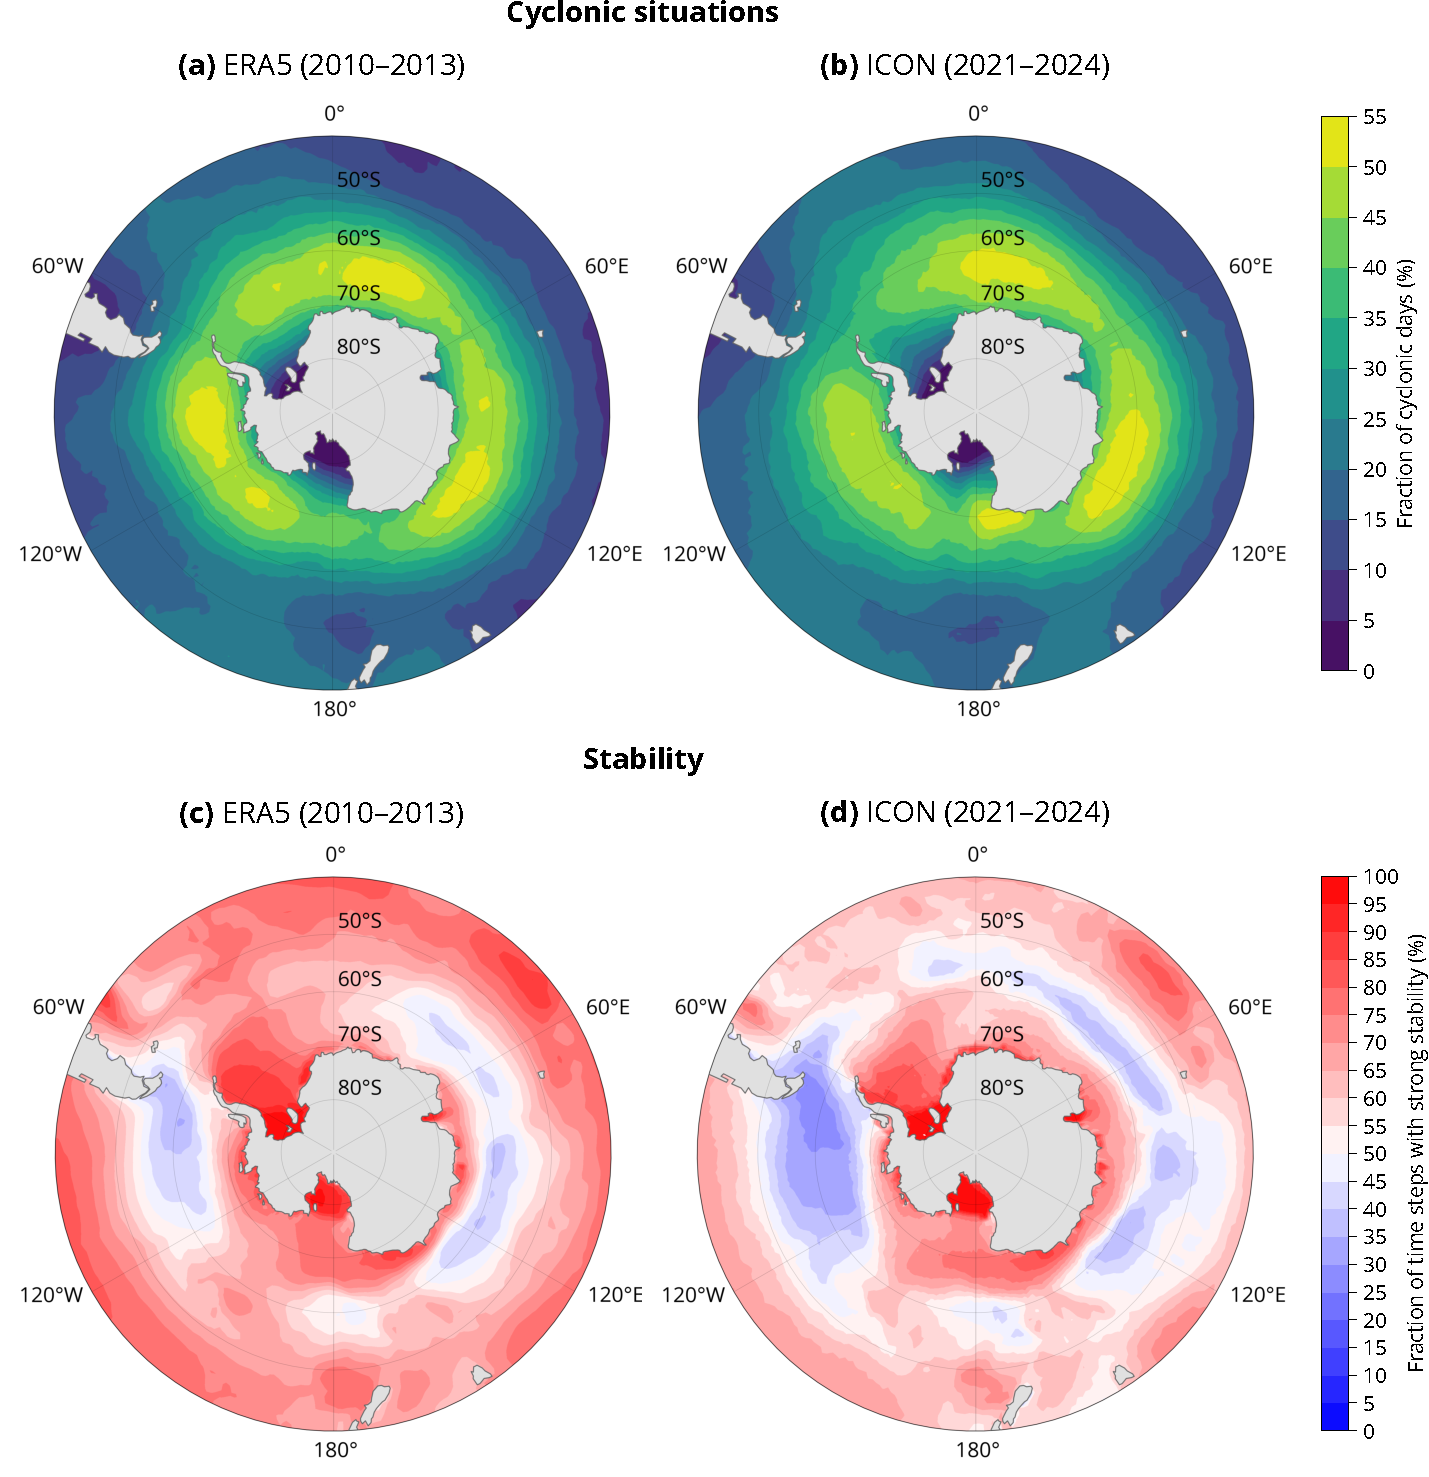
\includegraphics[width=\textwidth]{img/cyc_stab_dist.pdf}
\caption{
Geographical distribution of \textbf{(a, b)} cyclonic days and \textbf{(b, d)}
relatively stable (LTS > 12 K) time steps in \textbf{(a, c)} ERA5 in years
2010--2013 (inclusive) and \textbf{(b, d)} ICON in model years 2021--2023 (free
running). Cyclonic days are expressed as a fraction of the number of days with
cyclonic activity, defined as grid points located within a double radius of any
cyclone on a given day (UTC), as identified by CyTRACK.
}
\label{fig:lts}
\end{figure}

\section{Methods}
\label{sec:methods}

\subsection{Voyage and station data}

Together, we analysed data from 31 voyages of RV \emph{Polarstern}, resupply
vessel (RSV) \emph{Aurora Australis}, RV \emph{Tangaroa}, RV \emph{Nathaniel B.
Palmer}, Her Majesty's New Zealand Ship (HMNZS) \emph{Wellington} and one
sub-Antarctic station (Macquarie Island) in the SO south of 40°S between 2010
and 2021. Fig. \ref{fig:map} shows a map of the voyages, Table \ref{tab:voyages}
list the voyages and stations, and \ref{tab:voyage-references} lists references
where available. Altogether, the voyages and station dataset comprised
2421 days of data south of 40°S, but the availability of ceilometer data was
slightly smaller due to gaps in measurements.

Missing days in the ceilometer data were HMNZSW16 (7 days): 24--27 November, 10
December, 16--17 December 2016; MARCUS (3 days): 8, 10 November, 10 December;
MICRE (9 days): 7--8, 29 June, 5, 16 July, 15 August, 17 October 2016, 11
February, 21 March 2017; TAN1502 (1 day): 24 January.

The data sources contained ceilometer observations captured by the Vaisala CL51
and CL31 operating at a wavelenght of 910 nm and the Lufft CHM-15k operating at
1064 nm, described in detail below (Sections \ref{sec:cl51} and
\ref{sec:chm15k}). A ceilometer is a low-power near-infrared vertically
pointing lidar with the purpose of measuring the cloud base, but it also
measures the full vertical structure of clouds as long as the laser signal is
not attenuated by thick clouds, which can be used to infer additional
information such as a cloud mask and cloud occurrence by height.

Apart from lidar observations, radiosondes were launched on weather balloons at
regular synoptic times on the RV \emph{Polarstern}, MARCUS, NBP17024, TAN1702,
and TAN1802 voyages, measuring pressure, temperature, relative humidity, and
global navigation satellite system coordinates. Derived thermodynamic (virtual
potential temperature, lifting condensation level, etc.) and dynamic physical
quantities (wind speed and direction) for the measured vertical profiles were
calculated with rstool \citep{rstool}. Surface meteorological quantities were
measured continuously by an onboard automatic weather station or individual
instruments.

\subsection{Vaisala CL51 and CL31}
\label{sec:cl51}

The Vaisala CL51 (photo in Fig. \ref{fig:map}d) and CL31 are ceilometers
operating at a near-infrared wavelength of 910 nm. The maximum range is 15.4 km
(CL51), 7.7 km (CL31 with 5 m vertical resolution), and 7.550 km (CL31 with 10
m vertical resolution). The vertical resolution is 10 m (5 m configurable), and
the sampling (temporal) resolution is 6 s (AA15‐16, MARCUS, and MICRE), 36 s (RV
\emph{Polarstern}), and about 2.37 s (TAN1502). From the MARCUS voyage, unlike raw
instrument data available for the other voyages and stations, the Vaisala CL31
data were made available by the Atmospheric Radiation Measurement (ARM)
processed to a maximum range of 7.545 km, a vertical resolution of 30 m, and
sampling resolution of 16 s. The wavelength of 910 nm is affected by water
vapour absorption of about 20\% in the mid-latitudes
\citep{wiegner2015,wiegner2019}.  The instrument data files containing raw
uncalibrated backscatter were first converted to NetCDF with cl2nc
(\url{https://github.com/peterkuma/cl2nc}) and then processed with the ALCF
(Section \ref{sec:alcf}) to produce absolutely calibrated attenuated volume
backscattering coefficinet (AVBC), cloud mask, cloud occurrence by height and
the total cloud fraction. CL51 can also be configured to emulate CL31. The
Vaisala CL51 and CL31 instruments were used on most of the voyages and stations
analysed here. Fig. \ref{fig:example}a shows an example of derived from the
CL51 instrument.

\subsection{Lufft CHM 15k}
\label{sec:chm15k}

The Lufft CHM 15k (photo in Fig. \ref{fig:map}c) is a ceilometer operating at a
near-infrared wavelength of 1064 nm. The maximum range is 15.4 km, the vertical
resolution is 5 m in the near range (up to 150 m) and 15 m above, the sampling
(temporal) resolution is 2 s, and the number of vertical levels is 1024.
NetCDF files containing uncalibrated backscatter produced by the instrument
were processed with the ALCF (Section \ref{sec:alcf}) to produce AVBC, cloud
mask, cloud occurrence by height and the total cloud fraction. The CHM 15k was
used on a minority of voyages (HMNZSW16, TAN1702, TAN1802, and NBP1704).

\subsection{ALCF}
\label{sec:alcf}

The Automatic Lidar and Ceilometer Framework (ALCF) is a ground-based lidar
simulator and a tool for processing observed lidar data, supporting various
instruments and models. It performs radiative transfer calculations to derive
equivalent lidar AVBC in an atmospheric model, which can then be compared with
observed AVBC \citep{kuma2021}. For this purpose, it takes atmospheric fields
of cloud fraction, liquid and ice mass mixing ratio, temperature, and pressure
fields as an input and can be run offline (on the model output rather than
inside the model code). The lidar simulator in the ALCF is based on the
instrument simulator Cloud Feedback Model Intercomparison Project (CFMIP)
Observation Simulator Package (COSP) \citep{bodas-salcedo2011}.  After AVBC is
calculated, a cloud mask, cloud occurrence by height, and the total cloud
fraction are determined. The ALCF has already been used by several research
teams for model and reanalysis evaluation
\citep{kuma2020,kremser2021,guyot2022,pei2023,whitehead2023,mcdonald2024}.

Absolute calibration of the observed backscatter was performed by comparing the
measured clear-sky molecular backscatter statistically with simulated clear-sky
molecular backscatter. AVBC is resampled to 5 min temporal resolution and 50 m
vertical resolution to increase signal-to-noise ratio, while having enough
resolution to detect small-scale cloud variability. Noise standard deviation is
calculated from AVBC at the highest range, where no clouds are expected.  A
cloud mask is calculated from AVBC using a fixed threshold of $\mathrm{2\times
10^{-6} m^{-1}sr^{-1}}$ after subtracting 5 standard deviations of range-scale
noise. Fig. \ref{fig:example}b shows an example of simulated Vaisala CL51
backscatter from ERA5 data, corresponding to a day of measurements by the
instrument on the PS81/3 voyage.

\subsection{ICON}

A coupled (atmosphere--ocean) GSRM version of the ICON model is in development
by the nextGEMS project \citep{hohenegger2023}. ICON is a very versatile model,
allowing for simulations ranging from coarse-resolution ESM simulations, GSRM
simulations, limited area model (LAM) simulations, to large eddy simulations
(LES), for both weather prediction and climate projections. ICON uses the
atmospheric component ICON-A \citep{giorgetta2018}, whose physics is derived
from ECHAM6 \citep{stevens2013}, and the ocean component ICON-O
\citep{korn2022}. Earlier runs of the GSRM ICON from DYAMOND were evaluated by
\cite{mauritsen2022}.

Here, we use a free running (i.e. \emph{not} nudged or using prescribed SST)
coupled GSRM simulation made for the purpse of climate projection.  nextGEMS
has so far produced four cycles of model runs. We used a Cycle 3 run
\emph{ngc3028} produced in 2023 \citep{nextgems2023a,nextgems2023b} for a model
time period of 20 January 2020 to 22 July 2025, of which we analysed the full
years 2021--2024 (inclusive). While a Cycle 4 run was available, we could not
use due it to the unavailability of the necessary variables. The horizontal
resolution of ngc3028 is about 5 km.  The model output is available on 90
vertical levels and 3-hourly instantaneous temporal resolution.  Unlike current
general circulation models (GCMs), the strom-resolving version of ICON does not
use convective and cloud parameterisation but relies on explicit simulation of
convection and clouds on the model grid. While this makes the code development
simpler without having to rely on uncertain parameterisations, it can miss
smaller-scale clouds below the grid resolution.  Turbulence and cloud
microphysics are still parameterised in this model.

Because the model is free-running, weather and climate oscillations (such as
the El Niño--Southern Oscillation) are not expected to be equivalent to reality
at the same time and place. To compare with the observations collected on
different years (2010--2021, inclusive), we compared the model output with
observations at the same time of year and geographical location, as determined
for each data point such as a lidar profile or a radiosonde launch.

\subsection{MERRA-2}

The Modern-Era Retrospective analysis for Research and Applications, Version 2
(MERRA-2) is a reanalysis produced by the Global Modeling and Assimilation
Office at the NASA Goddard Space Flight Center \citep{gelaro2017}.  It uses
version 5.12.4 of the Goddard Earth Observing System (GEOS) atmospheric model
\citep{rienecker2008,molod2015}. The reanalysis output analysed here is
available at a spatial resolution of 0.5° of latitude and 0.625° of longitude,
which is about 56 km in the North--South direction and 35 km in the East--West
direction at 60°S. The number of vertical model levels is 72. Here, we use the
following products: 1-hourly instantaneous 2D single-level diagnostics
(M2I1NXASM) for 2-m temperature and humidity; 3-hourly instantaneous 3D
assimilated meteorological fields (M2I3NVASM) for cloud quantities, pressure,
and temperature; 1-hourly average 2D surface flux diagnostics (M2T1NXFLX) for
precipitation and sea ice; and 1-hourly average 2D radiation diagnostics
(M2T1NXRAD) for radiation quantities \citep{merra2}.

\subsection{ERA5}

ERA5 \citep{era5} is a reanalysis produced by the European Centre for
Medium-Range Weather Forecasts (ECMWF). It is based on a numerical weather
prediction (NWP) model Integrated Forecast System (IFS) version CY41R2.  The
horizontal resolution is 0.25° in latitude and longitude, which is about 28 km
in the North--South direction and 14 km in the East--West direction at 60°S.
Internally, the model uses 137 vertical levels. Here, we use output at 1-hourly
instantaeous time intervals, except for radiation quantities, which are
accumulations (from these we calculate daily means).  Vertically-resolved
quantities are made available on 37 pressure levels.

\subsection{CERES}

TOA radiation quantities are taken from the Clouds and the Earth’s Radiant
Energy System (CERES) instruments on board of the Terra and Aqua satellites
\citep{wielicki1996,loeb2018}. In our analysis we use the adjusted all sky SW
and LW upwelling fluxes at TOA from the synoptic TOA and surface fluxes and
clouds 1 degree daily edition 4A product
(CER\_SYN1deg-Day\_Terra-Aqua-MODIS\_Edition4A)
\citep{doelling2013,doelling2016}.

Radiation calculations presented in the results (Section \ref{sec:results})
were done in such a way that they always represent averages of daily means.
This is done in order to be consistent with the CERES SYN1deg data, which are
available as daily means. Therefore, every instantaneous profile in the
simulated lidar data is assigned a daily mean radiation value corresponding to
the day (in the Coordinated Universal Time; UTC). In turn, the average
radiation during the entire voyage or station observation period is calculated
as the average of the profile values. In the observed lidar data, the daily
mean radiation value is taken from the spatially and temporally co-located
CERES SYN1deg data of the day (in UTC). The voyage or station average is
calculated in the same way.

\subsection{Precipitation identification using machine learning}
\label{sec:ann}

Precipitation can cause strong enough lidar backscattering to be recognised as
a cloud by the threshold-based cloud detection method used in the ALCF. This is
undesirable if equivalent precipitation backscatter is not included in the
simulated lidar profiles. It was not possible to include precipitation
simulation in the ALCF due to the absence of required fields in the ICON model
output and the reanalysis data (the liquid and ice precipitation mass mixing
ratios), and because the required radiation calculations for precipitation are
currently not implemented in the ALCF. In order to achieve a fair comparison of
observations with models, one should exclude observed and simulated lidar
profiles with precipitation either manually or using an automated method. It is
relatively difficult to distinguish precipitation backscatter from cloud
backscatter in lidar observations, especially when only one wavelength channel
and no polarised channel are available. In models, the same can be accomplished
relatively easily by excluding profiles exceeding a certain amount of surface
precipitation flux. In the observations, using precipitation flux measurements
from rain gauges can be very unreliable on ships due to ship movement and
turbulence caused by nearby ship structures. Our analysis of rain gauge data
from the RV \emph{Tangaroa} showed large discrepancies between the rain gauge
time series and human-performed synoptic observations, as well as large
inconsistencies in the rain gauge time series. Human-performed observations of
precipitation presence or absence are expected to be reliable, but only cover a
limited set of time instants. Therefore, it was desirable to implement a method
of detecting precipitation from observed backscatter profiles alone.

On the RV \emph{Polarstern} voyages, regular human-performed synoptic
observations were available and included precipitation presence or absence and
type. We used this dataset to train a convolutional artificial neural network
(ANN) of the U-Net type \citep{ronneberger2015} to recognise profiles with
precipitation from lidar backscatter (Fig. \ref{fig:ann}a), implemented in the
TensorFlow ANN framework \citep{tensorflow}. Samples of short time intervals
(10 min) of near-surface lidar backscatter (0–250 m) were classified as clear,
rain, snow, and fog, using the synoptic observations as a training dataset
(Fig.  \ref{fig:ann}b). From these, a binary, mutually exclusive classification
of profiles as precipitating (rain or snow) or dry (clear or fog) was derived.
For detecting model and reanalysis precipitation, we used a fixed threshold for
surface precipitation flux of 0.1 mm h$^{-1}$ (the ANN was not used).

The ANN achieved 65\% sensitivity and 87\% specificity when the true positive
rate (26\%) was made to match observations. The receiver operating
characteristic curve is shown in Fig. \ref{fig:ann}c. We considered these rates
satisfactory for the purpose of filtering precipitation profiles. Fig.
\ref{fig:ann}d shows examples of the predicted precipitation compared to
human-performed observations.

\subsection{Partitioning by cyclonic activity and stability}

We partitioned our data into two subsets by cyclonic activity. For this
purpose, we used a cyclone tracking algorithm to identify extratropical and
polar cyclones (ECs and PCs) over the SO in the reanalysis and ICON data. We
used the open source cyclone tracking package CyTRACK
\citep{perez-alarcon2024}.  Generally, what constitutes an EC is considered
relatively arbitrary due to the very large variability of ECs \citep{neu2013}.
We used the mean sea level pressure field and horizontal wind speed fields as
input to the CyTRACK algorithm. The algorithm uses pressure and wind speed
thresholds as well as tracking across time steps to identify cyclone centres
and radii. From this information, we could classify geographical areas as
either cyclonic or non-cyclonic. Due to a relatively small total area covered,
we chose a circle of a double radius (relative to one identified by CyTRACK)
centred at the cyclone centre as a cyclonic area for every time step and
cyclone. All other areas were identified as non-cyclonic. For identifying
cyclones in the observations and the reanalyses, ERA5 pressure and wind fields
were used as the input to CyTRACK.  This is justified by the fact that the
large-scale pressure and wind fields in ERA5 are likely sufficiently close to
reality. For identifying cyclones in ICON, its own pressure and wind fields
were used as the input to CyTRACK, because the model is free-running, and thus
the pressure and wind fields are different from reality.

In addition to the above, we partitioned our data into two subsets by
stability. We determined this by calculating lower tropospheric stability (LTS)
as the difference between the potential temperature at 700 hPa and the surface.
Based on a histogram of LTS in ERA5 and MERRA-2 calculated at all voyage tracks
and stations (Fig.  \ref{fig:lts}), we determined a dividing threshold of 12 K
for relatively unstable (< 12 K) and relatively stable (>= 12 K) conditions.

\section{Results}
\label{sec:results}

\begin{table}
% TODO: Add sampling intervals.
\caption{
List of voyages and stations. Start, end, and days (UTC; inclusive)
indicate the time period when the vessel was south of 40°S. Abbreviations:
ceilometer (ceil.), Australia (AU), New Zealand (NZ), South America (SA),
Atlantic Ocean (AO) and Africa (AF). The number of days is rounded to the
nearest integer. CL51/31 indicates CL51 configured to emulate CL31.
}
\label{tab:voyages}
\small
\begin{tabular}{llllllr}
\textbf{Name} & \textbf{Vessel or station} & \textbf{Ceil.} & \textbf{Region} & \textbf{Start} & \textbf{End} & \textbf{Days}\\
\hline
AA15-16  & RSV \emph{Aurora Australis}   & CL51    & AU       & 2015-10-22 & 2016-02-22 & 124 \\
HMNZSW16 & HMNZS \emph{Wellington}       & CHM 15k & NZ       & 2016-11-23 & 2016-12-19 & 27 \\
MARCUS   & RSV \emph{Aurora Australis}   & CL31    & AU       & 2017-10-29 & 2018-03-26 & 149 \\
MICRE    & Macquarie Is. station         & CL51    & AU/NZ    & 2016-04-03 & 2018-03-14 & 710 \\
NBP1704  & RV \emph{Nathaniel B. Palmer} & CHM 15k & NZ       & 2017-04-14 & 2017-06-08 & 55 \\
PS77/2   & RV \emph{Polarstern}          & CL51    & SA/AO/AF & 2010-12-01 & 2011-02-04 & 65 \\
PS77/3   & RV \emph{Polarstern}          & CL51    & SA/AO/AF & 2011-02-07 & 2011-04-14 & 66 \\
PS79/2   & RV \emph{Polarstern}          & CL51    & SA/AO/AF & 2011-12-06 & 2012-01-02 & 27 \\
PS79/3   & RV \emph{Polarstern}          & CL51    & SA/AO/AF & 2012-01-10 & 2012-03-10 & 61 \\
PS79/4   & RV \emph{Polarstern}          & CL51    & SA/AO/AF & 2012-03-14 & 2012-04-08 & 26 \\
PS81/2   & RV \emph{Polarstern}          & CL51    & SA/AO/AF & 2012-12-02 & 2013-01-18 & 47 \\
PS81/3   & RV \emph{Polarstern}          & CL51    & SA/AO/AF & 2013-01-22 & 2013-03-17 & 55 \\
PS81/4   & RV \emph{Polarstern}          & CL51    & SA/AO/AF & 2013-03-18 & 2013-04-16 & 30 \\
PS81/5   & RV \emph{Polarstern}          & CL51    & SA/AO/AF & 2013-04-20 & 2013-05-23 & 33 \\
PS81/6   & RV \emph{Polarstern}          & CL51    & SA/AO/AF & 2013-06-10 & 2013-08-12 & 63 \\
PS81/7   & RV \emph{Polarstern}          & CL51    & SA/AO/AF & 2013-08-15 & 2013-10-14 & 60 \\
PS81/8   & RV \emph{Polarstern}          & CL51    & SA/AO/AF & 2013-11-12 & 2013-12-14 & 31 \\
PS81/9   & RV \emph{Polarstern}          & CL51    & SA/AO/AF & 2013-12-21 & 2014-03-02 & 71 \\
PS89     & RV \emph{Polarstern}          & CL51    & SA/AO/AF & 2014-12-05 & 2015-01-30 & 56 \\
PS96     & RV \emph{Polarstern}          & CL51    & SA/AO/AF & 2015-12-08 & 2016-02-14 & 68 \\
PS97     & RV \emph{Polarstern}          & CL51    & SA/AO/AF & 2016-02-15 & 2016-04-06 & 52 \\
PS103    & RV \emph{Polarstern}          & CL51    & SA/AO/AF & 2016-12-18 & 2017-02-02 & 46 \\
PS104    & RV \emph{Polarstern}          & CL51    & SA/AO/AF & 2017-02-08 & 2017-03-18 & 39 \\
PS111    & RV \emph{Polarstern}          & CL51    & SA/AO/AF & 2018-01-21 & 2018-03-14 & 52 \\
PS112    & RV \emph{Polarstern}          & CL51    & SA/AO/AF & 2018-03-18 & 2018-05-05 & 49 \\
PS117    & RV \emph{Polarstern}          & CL51    & SA/AO/AF & 2018-12-18 & 2019-02-07 & 51 \\
PS118    & RV \emph{Polarstern}          & CL51    & SA/AO/AF & 2019-02-18 & 2019-04-08 & 50 \\
PS123    & RV \emph{Polarstern}          & CL51    & SA/AO/AF & 2021-01-10 & 2021-01-31 & 21 \\
PS124    & RV \emph{Polarstern}          & CL51    & SA/AO/AF & 2021-02-03 & 2021-03-30 & 55 \\
TAN1502  & RV \emph{Tangaroa}            & CL51/31 & NZ       & 2015-01-20 & 2015-03-12 & 51 \\
TAN1702  & RV \emph{Tangaroa}            & CHM 15k & NZ       & 2017-03-09 & 2017-03-31 & 23 \\
TAN1802  & RV \emph{Tangaroa}            & CHM 15k & NZ       & 2018-02-07 & 2018-03-20 & 41 \\
\hline
\textbf{Total} &                         &         &          &            &            & \textbf{2421}\\
\end{tabular}
\normalsize
\end{table}

\begin{table}
\caption{List of voyage and station references.}
\label{tab:voyage-references}
\small
\begin{tabular}{lp{14.5cm}}
\textbf{Name} & \textbf{References}\\
\hline
AA15-16  & \cite{klekociuk2020} \\
MARCUS   & \cite{mcfarquhar2016,mcfarquhar2019,zhang2017,keeler2017,walton2017,cromwell2017,mcfarquhar2021} \\
MICRE    & \cite{marchand2015,marchand2020,zhang2016,mcfarquhar2021} \\
PS77/2   & \cite{kniglanglo2011a,kniglanglo2011b,kniglanglo2011c,kniglanglo2014a,fahrbach2011} \\
PS77/3   & \cite{kniglanglo2011d,kniglanglo2011e,kniglanglo2012a,kniglanglo2014b,knust2011} \\
PS79/2   & \cite{kniglanglo2012b,kniglanglo2012c,kniglanglo2012d,kniglanglo2014c,kattner2012} \\
PS79/3   & \cite{kniglanglo2012e,kniglanglo2012f,kniglanglo2012g,kniglanglo2014d,wolfgladrow2012} \\
PS79/4   & \cite{kniglanglo2012h,kniglanglo2012i,kniglanglo2012j,kniglanglo2014e,lucassen2012} \\
PS81/2   & \cite{kniglanglo2013a,kniglanglo2013b,kniglanglo2013c,kniglanglo2014f,boebel2013} \\
PS81/3   & \cite{kniglanglo2013d,kniglanglo2013e,kniglanglo2013f,kniglanglo2014g,gutt2013} \\
PS81/4   & \cite{kniglanglo2013g,kniglanglo2013h,kniglanglo2013i,kniglanglo2014f,bohrmann2013} \\
PS81/5   & \cite{kniglanglo2013j,kniglanglo2013k,kniglanglo2013l,kniglanglo2014g,jokat2013} \\
PS81/6   & \cite{kniglanglo2013m,kniglanglo2013n,kniglanglo2013o,kniglanglo2014h,lemke2013} \\
PS81/7   & \cite{kniglanglo2013p,kniglanglo2013q,kniglanglo2014i,kniglanglo2016a,meyer2013} \\
PS81/8   & \cite{kniglanglo2013r,kniglanglo2014j,kniglanglo2014k,kniglanglo2014l,schlindwein2014} \\
PS81/9   & \cite{kniglanglo2014m,kniglanglo2014n,kniglanglo2014o,kniglanglo2014p,knust2014} \\
PS89     & \cite{kniglanglo2015a,kniglanglo2015b,kniglanglo2015c,kniglanglo2015d,boebel2016}\\
PS96     & \cite{kniglanglo2016b,kniglanglo2016c,kniglanglo2016d,kniglanglo2016e,schrder2017} \\
PS97     & \cite{kniglanglo2016f,kniglanglo2016g,kniglanglo2016h,kniglanglo2016i,lamy2017} \\
PS103    & \cite{kniglanglo2017a,kniglanglo2017b,kniglanglo2017c,kniglanglo2017d,boebel2018} \\
PS104    & \cite{kniglanglo2017e,kniglanglo2017f,kniglanglo2017g,gohl2018,schmithsen2021a} \\
PS111    & \cite{schmithsen2019a,schmithsen2020a,schmithsen2021b,schmithsen2021c,schrder2018} \\
PS112    & \cite{schmithsen2019b,schmithsen2020b,schmithsen2021d,schmithsen2021e,meyer2018} \\
PS117    & \cite{schmithsen2019c,schmithsen2020c,schmithsen2021f,schmithsen2021g,boebel2019} \\
PS118    & \cite{schmithsen2019d,schmithsen2020d,schmithsen2021h,schmithsen2021i,dorschel2019} \\
PS123    & \cite{schmithsen2021j,schmithsen2021m,schmithsen2021n,schmithsen2021k,hoppmann2023} \\
PS124    & \cite{schmithsen2021o,schmithsen2021q,schmithsen2021p,hoppmann2023} \\
TAN1802  & \cite{kremser2020,kremser2021} \\
\end{tabular}
\end{table}

\begin{figure}
\centerline{
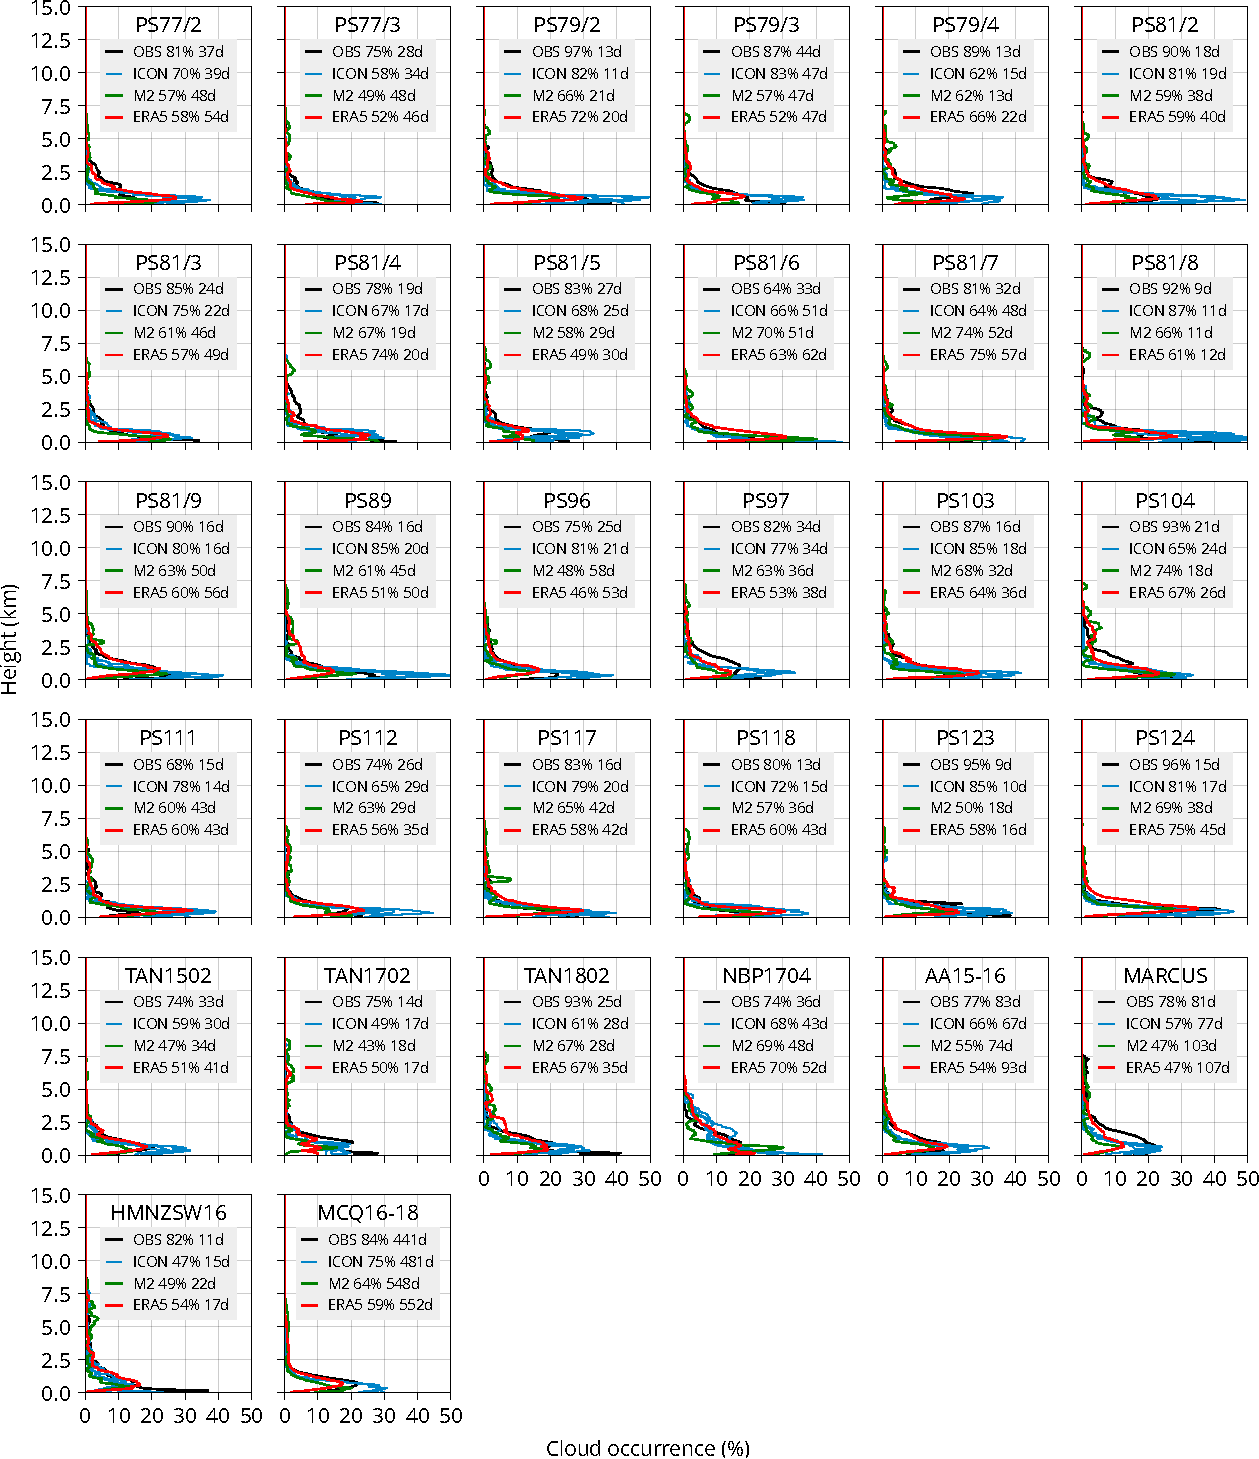
\includegraphics[width=1.06\textwidth]{img/cloud_occurrence_panel.pdf}
}
\caption{Cloud occurrence by height for the 31 voyages and one sub-Antarctic
station (MICRE) in observations (OBS), and simulated by the ALCF from the
ICON model, MERRA‐2 (M2) and ERA5 reanalysis data. The numbers in the legend
indicate the total cloud fraction and the number of days of data.}
\label{fig:cloud-occurrence-panel}
\end{figure}

\subsection{Cloud occurrence by height}

We used the ALCF to derive cloud occurrence by height and the total cloud
fraction from observations, ICON, and two reanalyses, MERRA-2 and ERA5 (Fig.
\ref{fig:cloud-occurrence-panel}). We aggregated the sources by calculating the
averages and percentiles of all individual profiles (Fig.
\ref{fig:cloud-occurrence}). The analysis shows that the total cloud fraction
(determined as the fraction of profiles with clouds at any height in the lidar
cloud mask) is underestimated in ICON and reanalyses by about 10\% and 20\%,
respectively.

In particular, ICON overestimates cloud occurrence below 1 km and
underestimates it above, MERRA-2 underestimates cloud occurrence at all
heights, especially near the surface, and ERA5 simulates cloud occurrence
relatively well above 1 km, but strongly underestimates it near the surface.
We note that fog or near-surface clouds are strongly lacking in the reanalyses.
As shown in Fig. \ref{fig:cloud-occurrence-panel}, the biases are relatively
consistent across voyages and longitudes. The ICON results are overall better
matching the observations than the reanalyses.

The ICON comparison is limited by the fact that the model is free-running.
Thus, the vertical profiles are not expected to represent the same weather
conditions as in observations, but long-term statistical comparison is still
possible. Only profiles with the same sea ice conditions (present or not) were
included to avoid comparing sea ice with open sea conditions.

The observations show cloud occurrence peaking at the surface, whereas models
show a higher peak (at about 500 m). The models underestimate total cloud
fraction by 10--20\% and show a strong decrease in cloud occurrence near the
surface, but this is not happening in the observations. ICON and ERA5
overestimate cloud occurrence at the peak (between 0--1 km). Above 1 km, ICON
and MERRA-2 understimate cloud occurrence, but ERA5 is very accurate. The too
high peak in models is partly supported by the LCL distribution, which peaks
higher in the models than in the observations (at the surface), although this
is not very pronounced. The northern zone shows a stronger peak of cloud
occurrence near the surface than the southern zone, and this could be because
higher latitudes have more unstable atmospheric profiles. The northern and
southern zones show similar biases in models as in the general case, but ERA5
does not overestimate the peak in the northern zone (near-surface cloud
occurrence is still strongly understimated). Cyclonic situations have a larger
amount of observed cloudiness, including the peak and total cloud fraction. In
these situations, the models are doing a relatively good job of getting the
vertical profile of cloud occurrence right, but still tend to underestimate
cloud occurrence above 1 km and near the surface. Non-cyclonic situations are
similar to the general case. In stable situations cloud occurrence peaks
strongly at the surface in observations, compared to unstable situations, where
the peak is more obtuse and spread across 0--1 km. In stable situations, the
models are doing a fairly good job, but overestimate cloud occurrence at the
peak below 1 km; above 1 km, they show similar biases as in the general case.
In unstable situations the bias in ICON is very pronounced, with a much
stronger peak at about 500 m, ERA5 is underestimating cloud occurrence below 1
km (especially near the surface), and MERRA-2 even more strongly. In all
situations, even when the models overestimate cloud occurrence at some
altitudes, they always substantially underestimate the total cloud fraction.
ICON can be generally characterised as substantially overestimating cloud
occurrence below 1 km and underestimating above, underestimating the total
cloud fraction, and showing greatest biases in unstable and non-cyclonic
condititions. It also shows a peak of cloud occurrence at higher altitude than
obs (500 m vs. near the surface), and correspondingly, its LCL tends to be also
higher. MERRA-2 can be generally characterised as underestimating cloud
occurrence at nearly all altitudes as well as the total cloud fraction, but
mostly above and below 500 m (the peak at 500 m is well-represented). It
struggles the most in the northern zone and in unstable situations. ERA5 can be
generally characterised as representing cloud occurrence correctly above about
1--1.5 km, overestimating below, but underestimating near-surface cloud
occurrence (0--500 m). The total cloud fraction is strongly understimated in
all situations. It has a tendency towards understimation in the northern zone
and unstable situations, conversely, overestimating in the southern zone and
stable conditions.

\begin{figure}
\centering
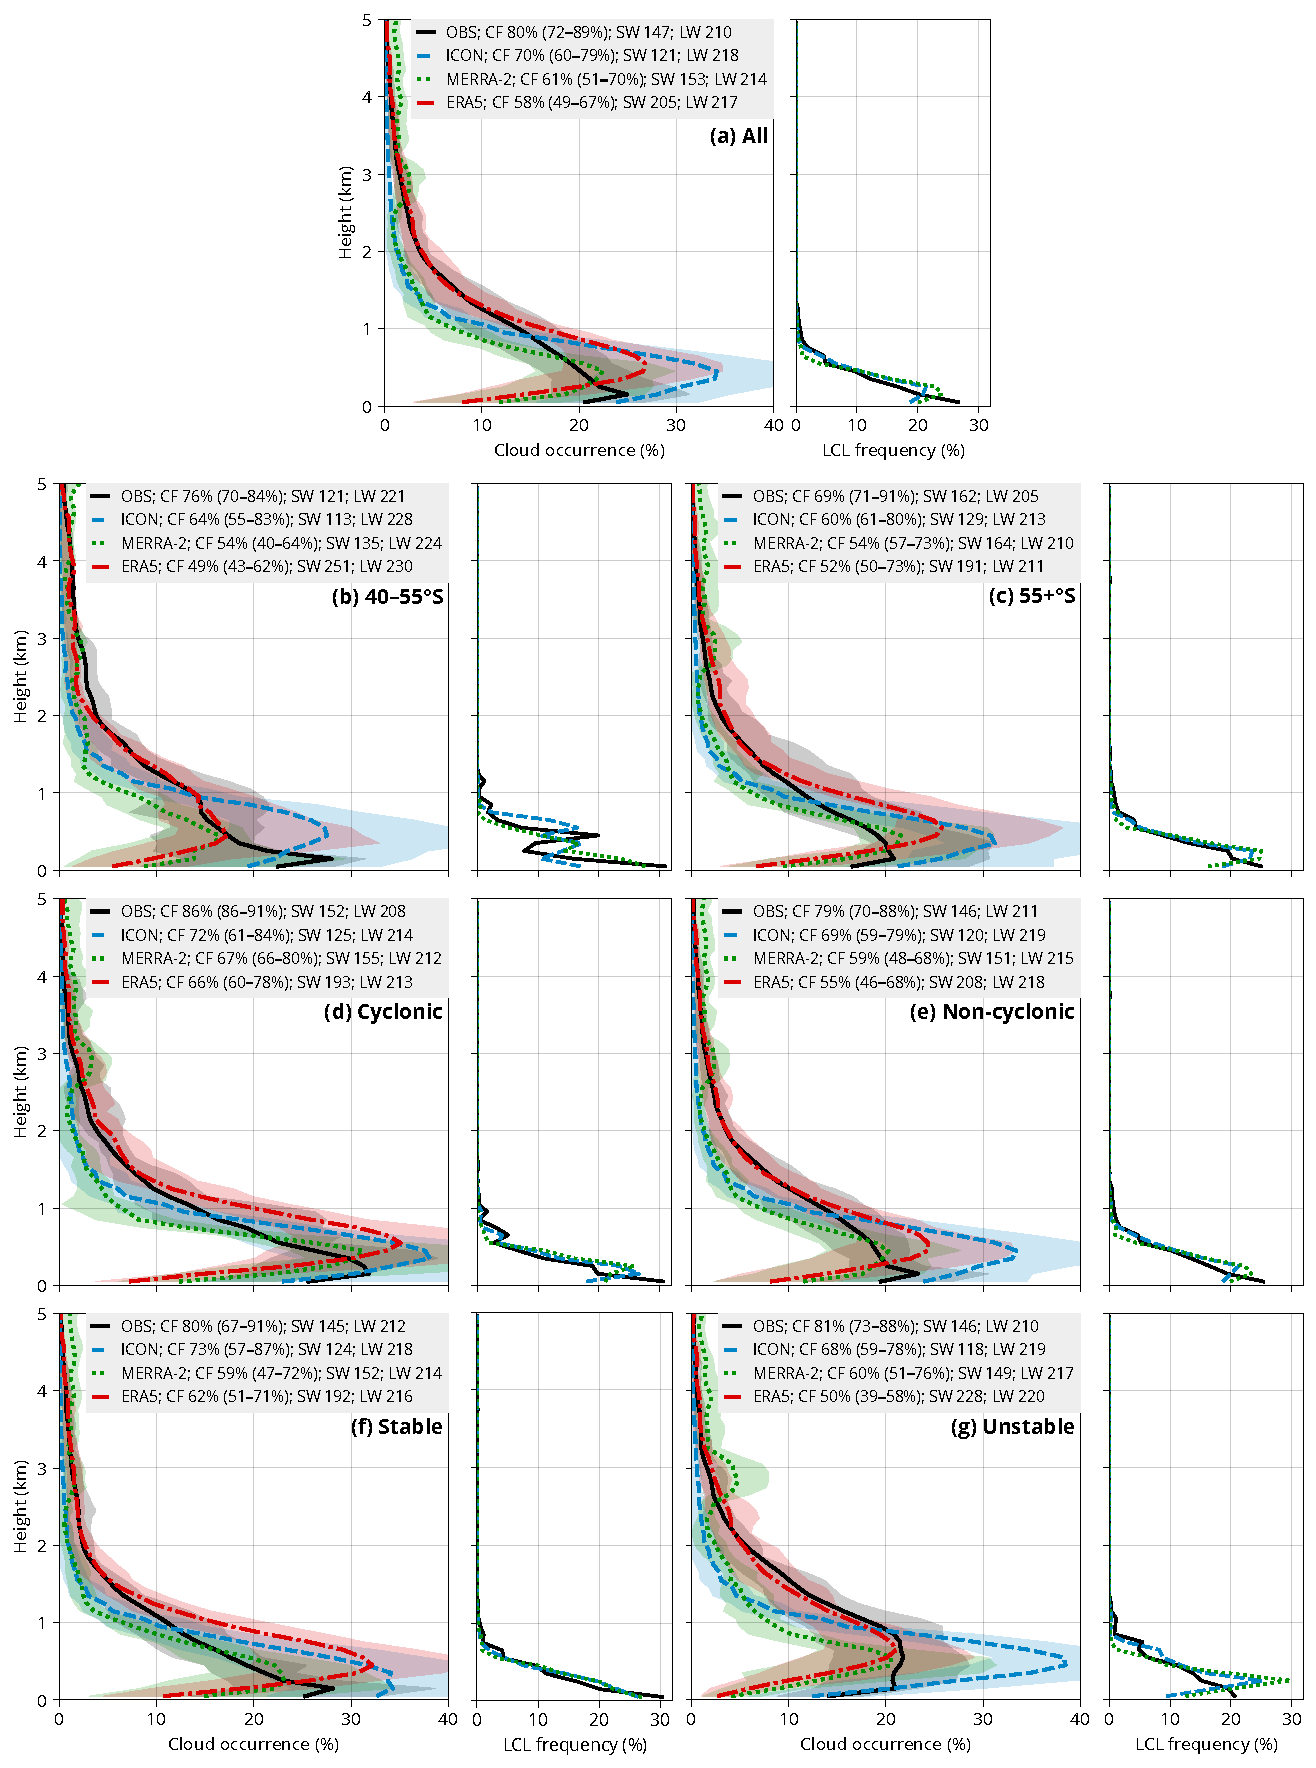
\includegraphics[width=\textwidth]{img/cl_agg.pdf}
\caption{
Cloud occurrence by height calculated as the average of all voyages and
stations for the observed (OBS) and simulated lidar cloud mask. The total cloud
fraction (CF), average shortwave (SW) and longwave (LW) are shown in the
legend, and the relative frequency of occurrence (RFO) of the subset is shown
below.  The bands span the 16$^\mathrm{th}$--84$^\mathrm{th}$ percentile
calculated from the set of all voyages and stations. The subsets
\textbf{(a--g)} are described in the text (Section \ref{sec:results}).
}
\label{fig:cloud-occurrence}
\end{figure}

\begin{figure}
\centering
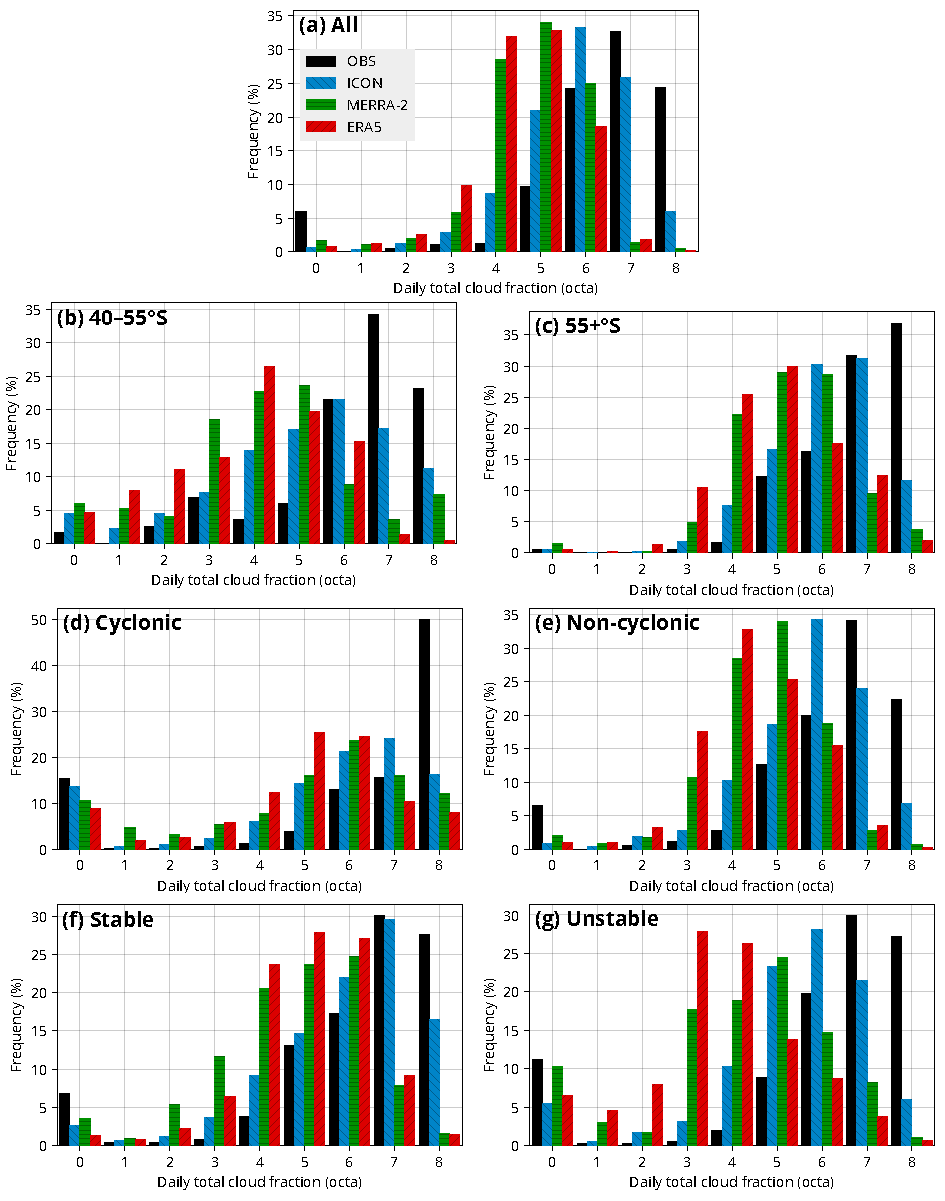
\includegraphics[width=\textwidth]{img/clt_hist.pdf}
\caption{
Daily total cloud fraction histograms calculated as the average of all voyage
and station histograms. The total cloud fraction of a day (UTC) is calculated
as a fraction of cloudy (based on the cloud mask) observed (OBS) or simulated
lidar profiles. The models and subsets are as in Fig.
\ref{fig:cloud-occurrence}.
}
\label{fig:cloud-cover}
\end{figure}

\subsection{Cloud cover}

We analysed the daily cloud cover (total cloud fraction) distribution. This is
a measure of cloudiness, irrespective of height. A cloud detected at any height
means that the lidar profile was classified as cloudy; otherwise, it was
classified as a clear sky. When all profiles in a day are aggregated together,
the cloud cover for the day is defined as the fraction of cloudy profiles in
the total number of profiles, expressed in octas.

In Fig.  \ref{fig:cloud-cover} we show the results for the same subsets as
analysed above. Observations show the greatest representation of high cloud
cover (5--8 octas), peaking at 7 octas. This is not represented by ICON or the
reanalyses.  While ICON is the closest, it tends to be 1 octa clearer the
observations, peaking at 6 octas, and highly understimating days with 8 octas.
Overall, the reanalyses show results similar to each other, underestimating
cloud cover by about 2 octas, and strongly understimating days with 7 and 8
octas. Of the two reanalyses, MERRA-2 shows slightly higher cloud cover and
thus more consistent with observations.

When analysed by subsets, the cyclonic subset shows the highest cloud cover,
with 8 octas occurring on one half of such days (Fig. \ref{fig:cloud-cover}d).
This is not represented by ICON or the reanalyses at all. Interestingly, clear
sky days (0 octas) also have a local maximum peaking at about 15\% in this
subset.  When we contrast the low and high latitude zones, we see that the high
latitude zone tends to have greater cloud cover, peaking at 8 octas (Fig.
\ref{cloud-cover}c). The high latitude also has almost no clear sky or small
cloud cover cases (0--4 octas). ICON and the reanalyses represent at least this
characteristic of the distribution well for 0--3 octas, but otherwise show
bises similar to the general case. One of the greatest biases is present in
ERA5 in the unstable subset, where it peaks at 3 octas, whereas the
observations peak at 7 octas and show negligible cloud cover below 5 octas.

\subsection{Thermodynamic profiles}

We analysed about 2300 radiosonde profiles south of 40°S from the 24 RV
\emph{Polarstern} voyages, MARCUS, NBP1704, TAN1702, and TAN1802. Spatially and
temporally colocated profiles were taken from ICON and the reanalyses. Because
the time period of the ICON model output was different from the observations,
model time was chosen to be the same as the radiosonde launch time relative to
the start of the year. The profiles were partitioned into the same subsets as
the lidar observations: all, 40--55°S, 55+°S, cyclonic, non-cyclonic, stable,
and unstable. The groups 40--55°S and 55+°S, cyclonic and non-cyclonic, and
stable and unstable were mutually exclusive in pairs. Apart from relative
humidity, we focus on comparing virtual potential temperature ($\theta_v$) due
to its role in low-level tropospheric stability, being one of the primary
factors affecting shallow convection and the associated low-level cloud
formation and dissipation. The observed and model profiles of virtual potential
temperature are shown in Fig. \ref{fig:potential-temperature}.

Overall, the mean $\theta_v$ is relatively well represented in ICON and
MERRA-2, being only slightly colder in the mid-to-high troposophere (less
stable) in ICON than in observations (Fig. \ref{fig:potential-temperature}a).
Large differences exist, however, in the 40--55°S zone, where ICON is colder in
$\theta_v$ by up to about 5 K and more so at higher altitudes (Fig.
\ref{fig:potential-temperature}b). In other subsets, the bias is relatively
small. MERRA-2 is very close to the observations, possibly due to a high
accuracy of assimilation of this quantity. Notably, the variability of virtual
potential temperature (as represented by the percentiles) is much smaller in
ICON than in the observations. This indicates that the model's internal
variability in the lower-tropospheric thermodynamic conditions in the SO is
smaller than in reality.

Relative humidity displays much larger biases. In all subsets, ICON is too
humid in the first 1 km, but very accorate above, except for the 40--55°S zone
and unstable conditions (Fig. \ref{fig:potential-temperature}b, g),  where it
is too dry between about 1 and 3 km. MERRA-2, on the other hand, is much more
humid than observations at all altitudes and in all subsets, by up to about
20\% at 5 km.

\begin{figure}
\centering
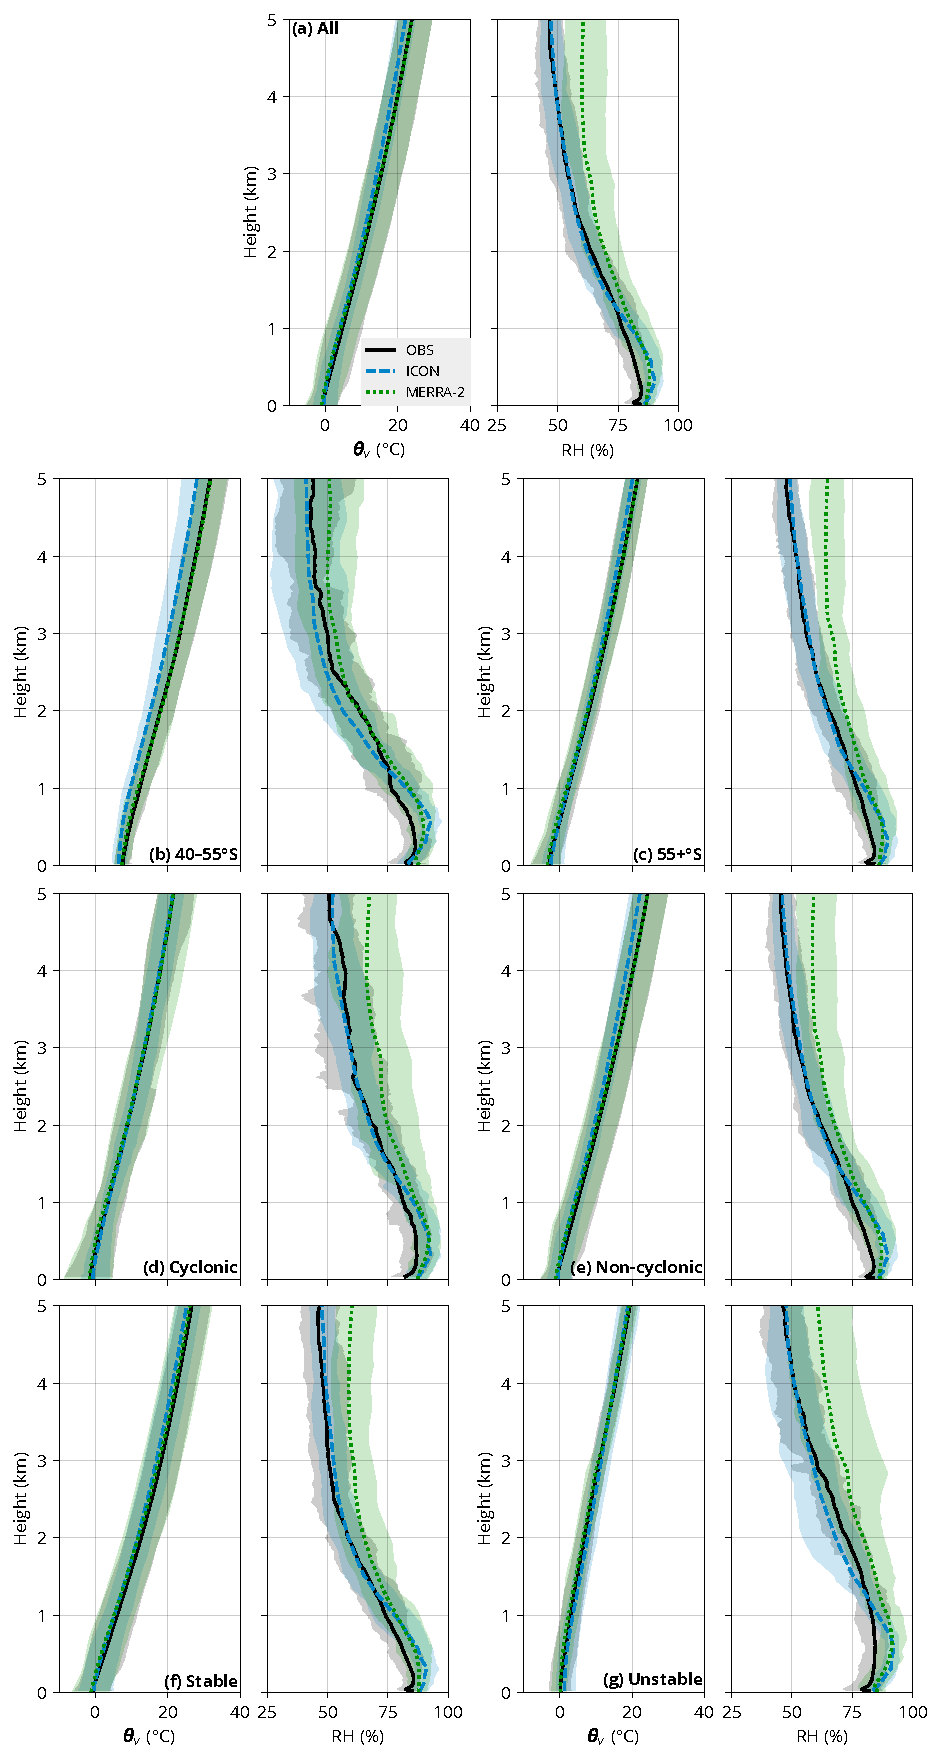
\includegraphics[width=0.72\textwidth]{img/theta_hur.pdf}
\caption{
Virtual potential temperature ($\theta_v$) and relative humidity (RH)
determined from radiosonde launches and co-located profiles in
ICON, ERA5, and MERRA-2 in subsets as in Fig. \ref{fig:cloud-occurrence}.
The solid lines are the average calculated from the averages of every
individual voyage and station. The bands span the
16$^\mathrm{th}$--84$^\mathrm{th}$ percentiles calculated from the distribution
of the voyage and station averages. Shown is also the relative frequency of
occurrence and the number of profiles in each subset.
}
\label{fig:potential-temperature}
\end{figure}

\section{Discussion and conclusions}

We show that the model underestimates the total cloud fraction by about 10\%,
with an overestimation of clouds below 2 km, and an underestimation of clouds
above 2 km. The reanalyses also underestimate the total cloud fraction by about
20\%.  ERA5 overestimates cloud below 1 km but underestimates near-surface
cloud or fog. In addition to lidar data, we compare radiosonde profiles
acquired on the RV \textit{Polarstern} voyages with ICON. Notably, the model
exhibits smaller natural variability than observations, and its lifting
condensation level tends to be higher. This might explain why cloud occurrence
is peaking higher in the model (at 500 m) than in observations (at the
surface).

Similar to our results, \cite{cesana2022} showed that CMIP6 also tends to
underestimate cloud occurrence above 2 km over the SO, although their analysis
in this case was limited to liquid clouds.

We compared radiosonde profiles acquired on the RV \emph{Polarstern} voyages
with ICON.  The ICON model exhibits smaller internal variability than
observations, and its LCL level tends to be higher, which might explain why a
peak of cloud occurrence in observations is located at the surface, while in
ICON it is located higher, corresponding to the LCL.

The results imply that SO cloud biases are still a significant issue in a
km-scale resolution model, even though an improvement over the lower-resolution
reanalyses is notable. More effort is needed to improve model cloud simulations
in this fast-changing and understudied region. The advancement from convection
and cloud parameterisation to cloud-resolving models might not solve this bias
without additional effort.

Further analysis will focus on investigating the role of cyclones in the
identified biases by using cyclone tracking and the role of local thermodynamic
stability using lower tropospheric stability and estimated inversion strength.

\section*{Acknowledgements}

We acknowledge the RV Polarstern datasets provided by the Alfred Wegener
Institute, RSV Aurora Australis datasets provided by the Australian Antarctic
Program and the University of Canterbury (UC), RV Tangaroa datasets provided by
the National Institute of Water and Atmospheric Research and the UC, RV
Nathaniel B. Palmer dataset provided by the National Science Foundation,
Cooperative Institute for Research in Environmental Sciences, University of
Colorado and the UC, HMNZS Wellington dataset provided by the Royal New Zealand
Navy and the UC and a Macquarie Island dataset provided by the Atmospheric
Radiation Measurement and the UC. We thank the scientific staff, the crew, and
everyone involved in collecting data on the voyages and Macquarie Island,
especially Kelly Schick, Peter Guest, John J. Cassano, Simon Parsons, Graeme
Plank, Sally Garrett, Jamie Halla, Sean Hartery, Mike J.  Harvey, Simon P.
Alexander and Alex Schuddeboom. We acknowledge the reanalysis dataset ERA5
provided by the Copernicus Climate Change Service and MERRA-2 provided by the
Global Modeling and Assimilation Office. We also acknowledge the AMSR Unified
and SMMR and SSM/I-SSMIS datasets provided by the National Snow and Ice Data
Center.

\section*{Code availability}

The ALCF, cl2nc, rstool, lidar precipitation detection code, and our data
processing and plotting code are open source and available at
\url{https://alcf.peterkuma.net}, \url{https://github.com/peterkuma/cl2nc}, and
\url{https://github.com/peterkuma/rstool}, and
\url{https://github.com/peterkuma/alcf-precip},
\url{https://github.com/peterkuma/icon-so-2024}, respectively. CyTRACK is
available at \url{https://github.com/apalarcon/CyTRACK}.

\section*{Data availability}

The RV \emph{Polarstern} data are openly available from Pangaea
(\url{https://pangaea.de}). The MARCUS and Macquarie Island (MICRE) data are
openly available from the Atmospheric Radiation Measurement (ARM)
(\url{https://www.arm.gov}). The MERRA-2 data are openly available from the
NASA NASA Goddard Earth Sciences (GES) Data and Information Services Center
(DISC) (\url{https://disc.gsfc.nasa.gov/datasets?project=MERRA-2}).  The ERA5
data are openly available from the Copernicus Climate Data Store (CDS)
(\url{https://cds.climate.copernicus.eu}). The CERES products are available
from the project website (\url{https://ceres.larc.nasa.gov}) and the NASA
Atmospheric Science Data Centre
(\url{https://asdc.larc.nasa.gov/project/CERES}).  The other voyage and station
data are openly available on Zenodo (). Subsetted model and reanalysis data for
the voyage tracks and the station and data processed with the ALCF are openly
available on Zenodo ().

\footnotesize
\setlength{\bibsep}{0.0pt}
\bibliography{manuscript}

\end{document}
